\documentclass[12pt,a4paper]{article}\usepackage[]{graphicx}\usepackage[]{color}
%% maxwidth is the original width if it is less than linewidth
%% otherwise use linewidth (to make sure the graphics do not exceed the margin)
\makeatletter
\def\maxwidth{ %
  \ifdim\Gin@nat@width>\linewidth
    \linewidth
  \else
    \Gin@nat@width
  \fi
}
\makeatother

\definecolor{fgcolor}{rgb}{0.345, 0.345, 0.345}
\newcommand{\hlnum}[1]{\textcolor[rgb]{0.686,0.059,0.569}{#1}}%
\newcommand{\hlstr}[1]{\textcolor[rgb]{0.192,0.494,0.8}{#1}}%
\newcommand{\hlcom}[1]{\textcolor[rgb]{0.678,0.584,0.686}{\textit{#1}}}%
\newcommand{\hlopt}[1]{\textcolor[rgb]{0,0,0}{#1}}%
\newcommand{\hlstd}[1]{\textcolor[rgb]{0.345,0.345,0.345}{#1}}%
\newcommand{\hlkwa}[1]{\textcolor[rgb]{0.161,0.373,0.58}{\textbf{#1}}}%
\newcommand{\hlkwb}[1]{\textcolor[rgb]{0.69,0.353,0.396}{#1}}%
\newcommand{\hlkwc}[1]{\textcolor[rgb]{0.333,0.667,0.333}{#1}}%
\newcommand{\hlkwd}[1]{\textcolor[rgb]{0.737,0.353,0.396}{\textbf{#1}}}%

\usepackage{framed}
\makeatletter
\newenvironment{kframe}{%
 \def\at@end@of@kframe{}%
 \ifinner\ifhmode%
  \def\at@end@of@kframe{\end{minipage}}%
  \begin{minipage}{\columnwidth}%
 \fi\fi%
 \def\FrameCommand##1{\hskip\@totalleftmargin \hskip-\fboxsep
 \colorbox{shadecolor}{##1}\hskip-\fboxsep
     % There is no \\@totalrightmargin, so:
     \hskip-\linewidth \hskip-\@totalleftmargin \hskip\columnwidth}%
 \MakeFramed {\advance\hsize-\width
   \@totalleftmargin\z@ \linewidth\hsize
   \@setminipage}}%
 {\par\unskip\endMakeFramed%
 \at@end@of@kframe}
\makeatother

\definecolor{shadecolor}{rgb}{.97, .97, .97}
\definecolor{messagecolor}{rgb}{0, 0, 0}
\definecolor{warningcolor}{rgb}{1, 0, 1}
\definecolor{errorcolor}{rgb}{1, 0, 0}
\newenvironment{knitrout}{}{} % an empty environment to be redefined in TeX

\usepackage{alltt}
\usepackage{fullpage}
\usepackage{setspace}
    \doublespacing
%\usepackage[usenames,dvipsnames]{xcolor}
\usepackage{hyperref}
\hypersetup{
    colorlinks,
    citecolor=black,
    filecolor=black,
    linkcolor=blue,
    urlcolor=blue
}
\usepackage{dcolumn}
\usepackage{booktabs}
\usepackage{url}
\usepackage{tikz}
\usepackage{todonotes}
\usepackage[T2A]{fontenc}
\usepackage[utf8]{inputenc}
\usepackage[english]{babel}
\usepackage{graphicx}
\usepackage{caption}
\usepackage{subcaption}
\usepackage{afterpage}
\usepackage{xpatch}
\usepackage{csquotes}
\usepackage[style=authoryear, sorting=nyt, dashed=false, maxbibnames=99, backend=bibtex]{biblatex}
\renewbibmacro{in:}{%
  \ifentrytype{article}{}{\printtext{\bibstring{in}\intitlepunct}}}
\renewbibmacro*{volume+number+eid}{
    \printfield{volume}
    \setunit*{\addnbspace}% NEW (optional); there's also \addnbthinspace
    \printfield{number}
    \setunit{\addcomma\space}
    \printfield{eid}}
\DeclareFieldFormat[article]{number}{\mkbibparens{#1}}


\renewcommand*{\bibpagespunct}{\addcolon\space}
\addbibresource{mybib.bib}
\IfFileExists{upquote.sty}{\usepackage{upquote}}{}
\begin{document}





\title{Why are More Trade-Open Countries More Likely to Repress the Media?}

\author{Justin Murphy\\
University of Southampton}

\maketitle

\begin{singlespace}
\begin{abstract}
Why are more trade-open countries more likely to repress the media, even though media freedom is positively correlated with general indices of economic globalization? To resolve this surprisingly under-reported empirical puzzle, I argue that economic globalization exerts contradictory pressures on state-media relations. Economic liberalization of trade, foreign direct investment, and foreign portfolio capital should generate incentives for states to repress the media, as states seek to manage the domestic distributive conflicts engendered by economic openness. However, whereas international \emph{investors} have a stake in the transparency of foreign countries, international \emph{traders} do not. Thus trade openness should have a uniquely negative effect on media freedom, as investment counter-balances but trade enables the repressive tendency generated by liberalization. To test these expectations, I use a mixed-methods research design combining statistical analysis of all available country-years between 1960 and 2011 and within-case process-tracing on two hard cases: Argentina and Mexico in the 1990s. Trade openness is found to have a large and highly robust negative effect on media freedom, with a one standard deviation increase in trade openness leading to as much as a .5 decrease in the probability of media freedom. Several robustness checks including tests for reverse causality, Bayesian model averaging, and genetic matching, all suggest this relationship is not an artifact of omitted variables, outliers, endogeneity, model selection, or the non-random assignment of trade openness. The article has important implications for current research on the globalization-democracy nexus and the comparative politics of media. \footnote{Justin Murphy (\href{http://jmrphy.net}{jmrphy.net}, \href{http://twitter.com/jmrphy}{@jmrphy}) is Assistant Professor of Politics at University of Southampton. Comments, questions, and feedback are welcome and can be sent to \href{mailto:j.murphy@soton.ac.uk}{j.murphy@soton.ac.uk}.}

\end{abstract}
\end{singlespace}

\vspace{0.3cm}

Given the conventional wisdom that democratic political institutions drive economic openness \parencite{Milner:2005ci} and vice-versa \parencite{EICHENGREEN:2008gg}, it is surprising that since the 1970s, on average, those countries which have been more open to international trade have had lower levels of media freedom. Although overall economic globalization is positively correlated with media freedom around the world, the bivariate relationship between trade and media freedom is weakly negative. The bottom half of Figure 1 shows that for all available country-years between 1970 and 2011, those which engaged in higher levels of international trade had slightly more repressive media, on average, than those countries which were less open to international trade. This is true in both historically democratic and non-democratic countries, although the difference is most clear among countries with more democratic histories. Given the positive correlation found between media freedom and economic globalization as measured by the KOF index for overall economic globalization \parencite{Dreher:2008dg}, the coincidence of higher trade openness and greater media repression is a surprisingly under-reported empirical puzzle in international and comparative political economy.

\afterpage{
\begin{figure}[t]
    \caption{Media Freedom and Trade vs. General Economic Globalization, 1970-2011}
    \label{absolute}
    \begin{center}
\begin{knitrout}
\definecolor{shadecolor}{rgb}{0.969, 0.969, 0.969}\color{fgcolor}

{\centering 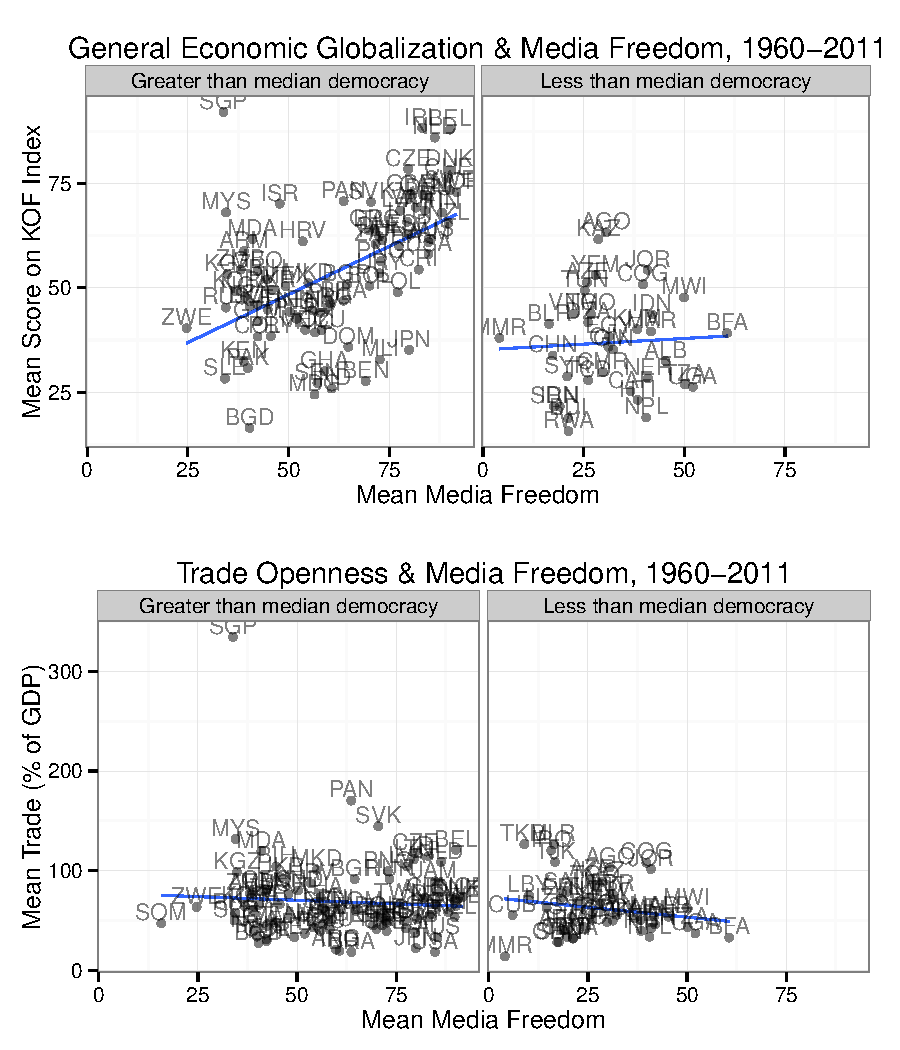
\includegraphics[width=\maxwidth]{figures/Intro} 

}



\end{knitrout}
    \end{center}
    \begin{singlespace}
        {\scriptsize{See the section on Data, Method, and Research Strategy for a more detailed description of the data sources. The KOF Index of Globalization (1970-2011) is a 100-point scale reflecting the quantity of international trade and investment policy restrictions as well as flows of trade, FDI, FPI, and income paid to foreign nationals and capital \parencite[43]{Dreher:2008dg}. Media freedom is measured on a dichotomous scale \parencites{Belle:1997wo}{van2000press}. Democracy refers to the 20-point scale from Polity IV \parencite{PolityIVProjectP:2011uq}.
                      }}
    \end{singlespace}
\end{figure}
\clearpage
}

This puzzle points to a larger gap in research on the domestic effects of economic globalization. Scholars of international and comparative political economy (IPE/CPE) have not yet developed a serious theoretical and empirical account of how national media politics are likely to be affected by increasing integration of national economies. Much is known about the effects of economic integration on aspects of domestic politics such as political cleavages \parencites{Rogowski:1987ip}{Rogowski:1989wm}{Hiscox:2002us}{hiscox2002international}, growth rates \parencite{Rodriguez:2001uw}; domestic spending \parencites{Rodrik:1998te}{Burgoon:2001dp}; civil war \parencites{Barbieri:2005uk}{Bussmann:2007vx}, and generic measures of democracy \parencites{EICHENGREEN:2008gg}{Li:2003vj}. But very little is known about how economic integration affects national media politics. One exception is a working paper by Orion Lewis \parencite*{Lewis:qDvYbWlU}, which finds mixed but suggestive evidence that trade openness is negatively related to media freedom and foreign direct investment (FDI) is positively related to media freedom. Other research has considered whether political and civil liberties (broadly including freedom of the media) affect international economic flows \parencite{Adam:2007gn} and the effect of media in economic reform \parencites{Coyne:2004bq}{Islam:2002uc}. Yet scholars of international and comparative political economy have not yet furnished any systematic analysis relating the different components and dynamics of globalization to the domestic politics of media freedom.

This article provides the first systematic investigation of how the various components of economic globalization--specifically, trade, FDI, and foreign portfolio investment (FPI)--shape the direction and dynamics of domestic media freedom. On the one hand, I argue that economic openness encourages national policymakers to promote media freedom because foreign investors are more likely to invest where information is reliable. On the other hand, because increasing globalization brings distributive conflict which can threaten governments, it also generates incentives for national policymakers to suppress information and communication. This paper outlines competing theoretical expectations from previous research and proposes a theoretical solution to reconcile these contradictory expectations. I argue that economic liberalization of trade and investment should increase the probability states will repress the media, as states seek to manage the domestic conflict it generates. However, while international \emph{investors} have a stake in the transparency of foreign countries, international \emph{traders} do not. Thus trade openness should have a negative effect on media freedom because, in contrast to investment, trade brings no pressures which would counter-balance the repressive tendency generated by liberalization.

To test these expectations, I use a mixed-methods research design combining statistical analysis of a large panel of countries from 1972 to 2003 and qualitative process-tracing on the cases of Argentina and Mexico.\footnote{For a full list of countries, see Table 3 in Supplementary Information.} Binary time-sectional, cross-series (BTSCS) analyses provide evidence that, unique among the components of globalization considered here, trade levels have a robustly negative association with media freedom in the long-run. Additionally, qualitative process-tracing on the cases of Argentina and Mexico in the 1990s, selected as relatively hard cases of consolidating democracies which for that reason predict media freedom, each provide some illustration of the mechanism relating trade openness to media repression.

The article makes three main contributions to research on the domestic effects of economic globalization and state-media relations. First, this article provides the first systematic investigation of an important but neglected set of relationships, placing a new set of questions regarding the globalization-media nexus into current political economy and media research agendas. Second, the findings contribute to research on the domestic politics of economic globalization and in particular research on the larger globalization-democracy nexus, highlighting when and how economic liberalization can call forth media repression as a troublingly anti-democratic technique for negotiating domestic political conflicts. Third, the article will be of interest to scholars of state-media relations and public actors interested in media freedom because very little media research to date has systematically accounted for the ways in which international economic pressures shape states' tendencies toward or away from media freedom.

The article proceeds in five sections. The first section reviews previous research at the intersection of globalization, democracy, and the media. The second section presents a simple informal model of a national policymaker facing domestic backlash for the distributive conflicts brought on by an increase in economic openness, and deducts one main hypothesis regarding the effect of trade openness on media freedom. The third section explains the data, methods, and research strategy. The fourth section presents and discusses the quantitative and qualitative findings, and the fifth section concludes.

\section{Globalization, Democracy, and Media}

Previous research provides strong reasons to expect the global integration of markets to exert pressures on institutions of democracy, but there remains much theoretical uncertainty about the degree to which these effects are positive or negative. Many have argued that economic globalization generates economic growth which strengthens democratic institutions \parencites{Baghwati:1997vy}{Im:1996cl}, increases incentives for peace \parencites{Baghwati:1997vy}{Oneal:1999fc}, or diffuses democracy as a norm (Kant [1795] \cite*{Kant:1983uf}; \cite{Limongi:1996dr}). On the other hand, many have argued that economic globalization is negatively associated with democracy because it rewards efficiency rather than popular sovereignty \parencites{Huntington:1975vt}{Lindblom:1977ue}{Cammack:1998gf}, or because leaders may prefer to repress rather than compensate the domestic losers from increased openness \parencite{Adsera:2002vt}.\footnote{See \cite{Milner:2009hi} for a review of these debates.} Within the general debate surrounding the globalization-democracy nexus, some researchers such as Li and Reveuny \parencite*{Li:2003vj} have sought greater clarity by disaggregating the distinct types of international economic flows and considering them separately, but relying on standard aggregate measures of democracy. Li and Reveuny find that trade and portfolio capital have negative effects on democracy, while FDI and democratic norms have a positive effect, but their dependent variable of democracy is calculated with the common procedure of subtracting the Polity autocracy score from the Polity democracy score. Thus, despite much research on the relationship between economic globalization and democracy, and despite evidence that disaggregation is fruitful for understanding this nexus of relationships, relatively little is known about how different international economic flows affect the various institutions which separately constitute what we know as democracy.

In particular, very little research to date queries whether and how economic globalization shapes state policies regarding domestic media freedom. One exception is Lewis \parencite*{Lewis:qDvYbWlU}, who finds that FDI inflows are positively associated with media freedom, trade levels are negatively associated with media freedom, and portfolio capital inflows have no discernible effect on media freedom. However, Lewis considers only levels of trade and year-by-year inflows of FDI and portfolio capital, whereas recent research shows that the distinction between flows (year-to-year movements) and stocks (the sum of all previous flows) is crucial in researching the effects of foreign investment on repression \parencite{Sorens:2012hc}. As discussed above, Antonis and Fillapaois \parencite*{Adam:2007gn} consider the effect of civil liberties such as media freedom on FDI, but not whether FDI affects civil liberties.

However, previous research on the relationship between markets and media more generally provides a basis for theorizing the relationship between economic integration and media freedom. Broadly, one tradition argues that the spread of markets and freer media are positively associated \parencites{Habermas:1991vg}{Islam:2002uc}{Islam:2003tu}. However, an opposite tradition suggets that markets and the logic of profits and efficiency create incentives for authoritarianism \parencite{Huntington:1975vt}. With respect to media politics in particular, Gehlbach and Sonin \parencite*{Gehlbach:2011ky} show that larger advertising markets are associated with nationalization of private media because, they argue, the benefits of state control increase with the advertising market. If economic liberalization tends to enlarge advertising markets by spurring economic growth, then liberalization might increase the state's incentives to repress private media just as it increases incentives to nationalize it. Furthermore, international economic integration brings the threat of social and political backlashes \parencite{Bussmann:2007vx}, which may require the state to compensate the domestic losers from globalization \parencite{Rodrik:1998te} or, alternatively, repress them \parencite{Adsera:2002vt}.

On the other hand, the literature on ``competitive authoritarianism'' suggests that increasing economic interdependence is one of the forces which has increasingly rendered traditional authoritarian repression unfeasible \parencite[60, 62]{Levitsky:2002gx}. As a country becomes increasingly integrated with the world economy, it increases the costs of overt authoritarianism by increasing the salience of international opinion, increasing the voice of domestic opposition, and increasing the number of domestic actors affected by international perceptions \parencite{Levitsky:2006ex}. For example, Fujimori in Peru in 1992 and Putin in Russia in 1993 failed in their efforts to overtly circumvent the legislature in part due to such international pressures \parencite[56]{Levitsky:2002gx}. International pressures against overt authoritarianism force regimes to adopt formally democratic institutions such as elections, but often leaves them free to violate human rights and civil liberties. For example, in the US-Mexico negotiations leading up to the North-American Free Trade Agreement, Mexican leaders made significant changes to present a front of democracy and respect for human rights to encourage investors, but there was no specific or formal conditionality which would have prohibited or even discouraged the repression of civil liberties if necessary.

At the same time, Levitsky and Way highlight the media as one of the four main arenas in which incumbent governments can contest and subvert international pressures to democratize. Competitive authoritarian governments may permit a formally independent and relatively free media, as in Peru, Serbia, Panama, or Nicaragua during the late 1980s and much of the 1990s, while engaging in alternative, more subtle tactics of repression, such as manipulative adminstrations of the law or tax code \parencite[53, 58]{Levitsky:2002gx}.

While economic integration engenders distributive conflicts which tempt states to repress certain domestic groups at the same time it disincentivizes certain overt techniques of repression, governments around the world increasingly engage in strategic, authoritarian interventions into domestic media politics. Corrales and Westhoff \parencite*{Corrales:2006vz} find, for instance, that authoritarian regimes are more likely to develop television than internet, because television is more easily controlled. Additionally, many authoritarian regimes welcome the internet but actively pursue techniques of information control and manipulation on the internet in a networked fashion \parencites{MacKinnon:2011id}{Pearce:2012fm}. These findings show that however much economic integration is making certain forms of repression obsolete, newer and more subtle techniques of media repression remain both attractive and viable.

As Antonis and Fillapaois point out, and as Lewis also argues, research on the relationship between globalization and democratic institutions likely shows such contradictory results because different international economic flows exert different pressures. To build on this idea while advancing the literature beyond the limitations discussed above, the next section provides a more deductive account of precisely why we should expect various types of international economic openness to exert different effects on media freedom.

The present study improves on the limited previous research in two ways. First, the present study uses newly expanded economic and media freedom data, which together permit the most comprehensive quantitative analysis of these relationships to date. In particular, I use the recently updated Global Media Freedom Dataset \parencites*{Belle:1997wo}{van2000press} and newly expanded measures of economic openness from Sorens and Ruger \parencite*{Sorens:wc} to analyze a large unbalanced panel of countries from 1960 to 2011. Second, I distinguish between levels and changes (long-run and short-run effects) in a country's exposure to international economic flows.

\section{Theory and Hypotheses}

Based on the review of previous research regarding the domestic political effects of international economic flows and the media politics of competitive authoritarianism, I develop a simple, informal model of how state media policy should respond to trade, FDI, and FPI. Consider a state which experiences a variable increase in some inward, international economic flow of trade, FDI, or FPI. This increased flow should increase the income of certain domestic groups and decrease the income of others, according to well-developed open-economy expectations (discussed below). The increased economic flow can be thought of as random and exogenous or the result of conscious state policy such as lowering tariffs. After experiencing the international shock, the media, if free to do so, would be expected to report on its causes and effects and therefore increasing public awareness of its distributive implications. Clearly, to the degree the media are not free to report on the international shock, they would not do so and public awareness of the distributive implications would remain lower than if the media had been free. If they are well-informed, a domestic group which experiences a negative income shock from economic liberalization would demand that the policymaker either close the domestic economy or compensate the group for its income loss, or else face rebellion. This “rebellion” could be electoral if the state is a democracy or a violent insurgency if the state does not have institutions to facilitate peaceful change. If the media is not free to report on the political context and consequences of the international shock, the group which suffers an income loss would be less likely to mobilize around it. In this simple informal model, it is easy to see why free media are essential for domestic losers from globalization to exercise power in the domestic politics around the distributive outcomes of economic globalization. Where there is a free media, domestic losers from globalization are more likely to hold policymakers accountable because they are more likely to be informed and more likely to mobilize around this issue. Where the media are repressed, the losers from globalization should be less able to exact concessions or compensations from policymakers because they will be less informed and therefore less mobilized around this issue.

After increased international exposure occurs, the policymaker would prefer not to compensate the domestic group but prefers compensation to facing rebellion or closing the economy to \emph{ex ante} levels. The policymaker can close the political process to any competitors to obviate the political pressure to compensate them \parencite{Adsera:2002vt}, but the higher their level of integration, the more costly are overt types of repression \parencite{Levitsky:2002gx}. Supposing that a policymaker can choose among compensating the aggrieved domestic group, excluding competitors from the political process, or engaging in some repressive practices which vary on a continuum from overt to covert. In effect, we can conceptualize their utility function as including a penalty on overtness which increases with the country's economic integration, such that there is decreasing utility to overt forms of repression such as outright exclusion from the political process or government killings but this disutility approaches zero for repressive tactics which are relatively obscure such as the selective prosecution or financial targeting of opponents.

Among the less visible ways of exercising anti-democratic control, information-communication control will be uniquely attractive for the policymaker. This is because not only are repressive media tactics less severe than mass killings or canceling elections, but because control of the media could potentially tame international judgments independently by shaping what gets reported internationally. That is, control of the media can first minimize policymaker accountability for the adjustment costs of liberalization by suppressing domestic dissent, but policymakers could also reasonably expect that suppressing information at home would decrease the flow of negative information abroad, promoting their international image in part by repressively shaping their image at home. In summary, increasing linkages to other states and international pressures raise the cost of overt repression for liberalizing states, which increases the attractiveness of more subtle, lower-visibility tactics for suppressing dissent against liberalization. Repression of the media stands out as a uniquely attractive first because it is precisely such a relatively low-visibility, low-salience type of repression but also because if successful it would tend to lower negative visibility in general.

\subsection{Differences among FDI, FPI, and trade}

The previous subsection argues that media repression is uniquely attractive to incumbents presiding over economic liberalization. However, the international actors who are the counterparties to a country's international exchanges are also strategic actors. When a government represses the flow of information and communication within its territory, these counterparties will respond strategically depending on how their particular investment in the country is affected by domestic freedom of information and communication. Given that these international counterparties have very different stakes in domestic media freedom depending on whether they are engaged in trade, foreign direct investment, or portfolio capital investment, the utility of media repression during economic liberalization will be conditioned according to a country's composition of exposure to these flows.

\subsection{FDI}

FDI is defined as the private capital flows from one firm to an enterprise located in a country outside of the firm's home nation. FDI flows consist of equity capital, intercompany debt, and reinvested earnings, whenever the investment is sufficient to give the firm a controlling stake (typically 10\%) in the enterprise \parencites[9]{DirectInvestmentTechnicalExpertGroupDITEG:2004wa}[588]{Jensen:2003to}. Foreign direct investment is unique among other types of international investment in that FDI involves a longer-term committment and thus the interests of FDI investors are relatively more aligned with the long-term interests of host countries \parencites{Lipsey:1999tn}[588]{Jensen:2003to}. The standard economic theory of FDI suggests that firm-level investment decisions to invest directly in a foreign country are not based on relative factor endowments or comparative rates of return, but on domestic market imperfections which can be exploited by multinational corporations (MNCs) better than domestic firms \parencites{Hymer:1960vo}{dunning2013international}. The distributive consequences of FDI inflows are complex: FDI is typically thought to increase inequality between skilled and unskilled workers as MNCs tend to be technologically skill-biased relative to domestic firms \parencite{Feenstra:1997kx} and unskilled, subsistence farmers do not have the resources to become entrepreneurs \parencite{Basu:2007ir}. However, FDI is also thought to decrease overall domestic income inequality as an increase in the supply of capital relative to labor increases wages and reduces inequality between capital and skilled labor \parencite{Jensen:2007fr}. Jensen and Rosas present evidence that, because poor countries have relatively little skilled labor, FDI's effect on closing the gap between skilled labor and capital is likely to decrease inequality on net even if it increases inequality between skilled and unskilled labor. Thus, FDI inflows generate distributive conflict among skilled and unskilled labor, but are unlikely to generate highly salient distributive conflict overall. This expectation is borne out by research on the relationship between economic globalization and civil war. Bussmann and Schneider \parencite*{Bussmann:2007vx} find, contrary to their expectations, that inflows of FDI decrease rather than increase the likelihood of civil war onset.

Of the three types of international economic actors considered here, investors of FDI have a long-term stake in the conditions of a host country. Because of this, despite long-standing expectations that foreign direct investors prefer the efficiency of authoritarian regimes, the balance of evidence suggests that democracies draw greater FDI flows than autocracies because they are more credible \parencite{Jensen:2003to}. Some scholars have sought to extend this logic by arguing that FDI should be attracted to respect for human rights \parencite{Blanton:2007gu} have faced problems of measurement and missing data \parencite{Sorens:2012hc}. After accounting for these issues, Sorens and Ruger find no link between FDI and human rights. Thus, while formal democracy attracts FDI and FDI does not appear to generate intense distributive conflicts, neither does it appear to “punish” governments for violating human rights. Antonis and Filipaios find, consistent with Jensen, that FDI seeks strong political rights while its attraction to civil rights is hump-shaped such that FDI is associated with both high and low levels of civil rights \parencite*{Adam:2007gn}. One possible explanation of these inconsistencies is that the socially positive consequences of FDI (rewarding democracy and rule of law and decreasing civil war onset) occur at the same time as, or perhaps in part through, the repression of civil rights. This is consistent with the model outlined above, wherein the repression of a particular civil right (the freedom of expression) embodied in media freedom is repressed to dampen the domestic conflict which would otherwise lead to perhaps more severe types of repression.

Thus, there are competing expectations regarding whether increases in FDI should be associated with media repression or media freedom. FDI does not appear averse to violations of rights per se, and may be attracted to governments with low respect for civil rights, so it possible FDI exerts no effect or a negative effect on media freedom, especially as its relative immobility means that its threat of exit would be less credible than that of FPI. On the other hand, FDI might be positively associated with media freedom for the same reasons it is associated with democracy, namely that it tends towards states which are credibile and stable.

\subsection{FPI}

FPI is defined as the purchase of stocks and bonds of less than 10\% of the outstanding stock of foreign firms \parencites{kenen1994exchange}{Walther:1997wf}. The standard economic theory is that portfolio capital tends to flow where the rate of return on the target country's domestic assets is high relative to the riskiness of the investment \parencites[743]{mosley2003global}[685]{ISQU:ISQU420}. Portfolio capital is distinguished, compared to FDI, by its short-term, speculative nature. In a benchmark study of how portfolio investors evaluate political risks, Bernhard and Leblang \parencite*{Bernhard:2003kb} show that portfolio investors respond to changes in country's political system (such as elections), but not to the substance of those changes (for instance, partisanship). Brooks and Mosley \parencite*{Brooks:2007we} show that portfolio investors do respond to the substance of policymaking, such as partisanship and macroeconomic priorities, but only in low-information environments such as electoral turnovers. The effects of partisanship and macroeconomic policy on portfolio capital decrease when the political system itself is stable. The overall point is that portfolio investors are first and foremost interested in stability and predictability rather than particular policies, which only matter in periods when the predictability of the future is low.

FPI inflows tend to appreciate the domestic currency, which makes imports relatively cheaper in the home market and exports relatively more expensive to foreigners. This will harm exports, leading possibly to unemployment or decreases in wage levels in export-intensive industries. It will also make it harder for domestic firms to compete with relatively cheaper imports, also possibly leading to unemployment or wage decreases. Finally, cheaper capital imports can encourage skill-biased shifts in technology usage, increasing the incomes of skilled labor and decreasing the incomes of unskilled labor \parencites{Cragg:1996iy}{Ros:2000vy}. Finally, because portfolio capital is relatively liquid, the threat of sudden withdrawal by international investors is well-known to have highly negative macroeconomic effects, such as in Mexico in 1995 and Argentina in 2001.

Given the interests of governments and portfolio investors, governments may be inclined to repress the media in response to the distributive effects of portfolio capital for two reasons. First, FPI inflows will make governments more beholden to the prevention of systemic political risks such as general strikes, expropriations, or revolutions \parencite{Clark:1997jg}. This is consistent with anecdotal evidence of portfolio investors who prefer governments to repress social unrest. Neoliberal economic reforms including international liberalization are often followed by large increases in FPI, and there is anecdotal evidence that in some cases foreign investors demand repression explicitly, such as when Chase Bank's Emerging Markets Group circulated a memo urging Mexican President Ernesto Zedillo to “eliminate the Zapatistas” and their uprising in Chiapas in 1994 \parencite{Silverstein:1995wc}.

Second, given that policy is evaluated by foreign investors largely in light of what is already known about the government and its history, incumbents who preside over financial liberalization may be sufficiently trusted by foreign capital that relatively subtle tactics such as media repression would be unlikely to shake confidence, especially if it is in the interest of preventing larger disruptions such as rebellions. It may be objected that portfolio investors would dislike media repression because they rely on a reliable flow of information regarding the country's conditions, but through modern “news management” politicians can practice a highly nuanced kind of transparency for international observers and also effectively repress domestic media using underhanded tactics. Indeed, country's which are open enough to receive capital inflows are likely to already be relatively transparent in the ways most relevant to investors, and this transparency required to induce investment might even embolden the assertiveness of domestic media. This appeared to happen in Mexico during the 1980s and 90s \parencite{lawson2002building}. Portfolio investors can typically rely on international news sources which are less likely to be targeted within the host country (on account of their financial independence and being linked to another sovereign, such as that one in Argentina). Finally, portfolio investors often have access to private, elite channels which provide them with politically important information about foreign country conditions before it would even be reported by free media \parencite{Dube:2011ir}, perhaps making them insensitive to media freedom within the host country.

Thus, there are competing expectations regarding the effects of FPI on media freedom, just as there are with respect FDI. As a country adjusts to the distributive effects of FPI, governments may be more likely to repress the media as a relatively discreet tactic of pacifying this conflict, consistent with investors' interests in stability. However, inflows of portfolio capital may in the long-run be associated with media freedom, as portfolio investors prefer high-information environments ceteris paribus. However, FPI is different from FDI in the crucial fact that it is more mobile and therefore represents a much more credible threat of exit in response to government behavior. Therefore, while the expectations regarding FDI and FPI are bi-directional, to the degree foreign investment has a disciplining effect on state-media relations favouring media freedom, this effect should be strongest for FPI.

\subsection{Trade}

Trade, defined simply as imports plus exports as the percentage of a country's gross domestic product, is unique among the previous two components of economic globalization in that the international counterparties have no direct economic stake in the social and political conditions of the home country. Put simply, trade is not an investment as are FDI and FPI. The standard economic intuition explaining trade flows, although many sophisticated variations and extensions have been developed, is still the well-known Ricardian theory of comparative advantage. Other things equal, countries will tend to specialize in producing for export those goods which they are most advantaged in producing, and import from foreign producers those goods which domestic producers are unable to produce as efficiently.

International trade theory and much research in political science provides well-established expectations regarding the distributive effects of a country increasing its exposure to international trade. The standard Stolper-Samuelson model (1941) expects that increasing trade openness increases the income of the domestically abundant factor while decreasing the income of the domestically scarce factor. Thus, in capital-rich countries (industrialized or post-industrial countries), increasing trade openness benefits capital and harms labor, whereas in capital-poor countries increasing trade openness is expected to benefit labor and harm capital owners. In his benchmark study on the political consequences of these distributive expectations, Rogowski \parencite*{Rogowski:1989wm} finds strong evidence that domestic political coalitions are empowered and disempowered by international trade as the Stolper-Samuelson model predicts. Hiscox \parencite*{Hiscox:2002us} further refines these expectations by showing that the history is more finely explained by distinguishing the relative mobility of factors: when domestic factors are relatively immobile within the domestic economy, we do not observe class-based cleavages but rather sector-based cleavages and cross-class alliances, as immobility weds the interests of labor and capital to their shared industry. In turn, the threat of distributive conflict from international trade has been found salient enough to explain domestic political outcomes as diverse as the size of welfare states \parencites{Cameron:1978vb}{Burgoon:2001dp} and the onset of civil wars \parencite{Bussmann:2007vx}.

The international counterparties to a country's international trade have a uniquely low stake in the political stability of the country, for the simple reason that the import and export of goods and services is not directly affected by the sanctity of civil rights such as freedom of expression or media freedom. Although emerging international norms of “corporate responsibility” and “fair trade” are increasingly visible in marketing for consumers in the wealthy democracies, these norms revolve around specific labor market issues such as child labor, ``sweatshops'', and wages paid to workers in developing countries \parencite{Moore:2004gy}. Even if some consumers in the wealthy democracies are increasingly willing to pay for more humane production conditions in foreign countries (effectively an international tax on repressive production conditions), there is no evidence and little reason to believe that economic behavior in importing or exporting goods and services anywhere in the world is in any way responsive to the sanctity of significantly less salient civil rights such as media freedom. For instance, consumers in the global North may very well prefer to pay premiums for coffee explicitly labeled as “fair trade,” but this provides no reason to expect they would pay more or less depending on whether the exporting country's trade agreements were facilitated by media repression. Similarly, if exporters in one country benefit from lowered tarrifs in a foreign country, compared to FDI and portfolio investors, they have uniquely less at stake in the political consequences faced by the foreign country with rising imports.

Thus, trade openness should be associated with a higher probability of media repression as it generates domestic distributive conflict but exerts little conceivable pressure in favor of a free media. If true, this would explain the puzzlingly negative correlation between international trade and media freedom despite the positive association between media freedom and most other components of economic globalization.

\subsection{Summary of Main Hypothesis}

To summarize, while theoretical expectations regarding the effects of FDI and FPI on media freedom are ambiguous, I have argued that trade openness is likely to have a uniquely negative effect on media freedom. Thus, for the present article I focus attention on testing one hypothesis, namely,

H1: Trade openness decreases the probability of media freedom.


\section{Data, Method, and Research Strategy}

To test the main hypothesis, this article pursues a mixed-method research design employing large-N statistical tests and qualitative within-case analysis on two historically important cases. The intuition behind this research strategy is that statistical analyses are necessary to disentangle the independent effects of each economic flow, while qualitative analysis is necessary for corroborating the existence of a causal process.

In the quantitative analyses, I use state-level economic data collected by Sorens and Ruger \parencite*{Sorens:wc} for the main independent variables of interest for all available countries between 1976 and 2003. $FDI$ and $FPI$ refer to logged stocks of each investment type, whereas $\Delta FDI$ and $\Delta FPI$ refer to changes in logged stocks (i.e., flows), all as percentages of GDP. $Trade$ and $\Delta Trade$ refer to levels and changes of international trade, respectively, also as percentages of GDP.   For the dependent variable, I use the Global Media Freedom Dataset by Whitten-Woodring and Van Belle \parencites*{van2000press}{Belle:1997wo}, which is the most comprehensive measure of media freedom to date. The Global Media Freedom Database provides an ordinal measure of media freedom with four levels but this variable reduces to a dichotomous variable capturing the distinction between not free and ``functionally free'' media. Country-years which take a value of ``not free'' are those where it is unsafe to criticize the government in the media or the government directly controls all news media. Countries which take a value of ``functionally free'' are those where there may be ``social, legal, or economic costs'' to criticizing the government in the news media but criticism of government still regularly takes place.\footnote{For greater detail, see ``Guidelines for using the Global Media Freedom Dataset'' available from the authors.}

To reduce the possibility of spurious results from omitted variables, the analysis includes a battery of control variables which are expected to shape the probability of media freedom independently of economic openness. First, it is well known that democratic institutions are positively associated with media freedom \parencite[13]{Islam:2008wj}. Economic development--especially through the mechanism of increasing financial independence from advertising revenue--is also a strong driver of media freedom \parencites{Petrova:2011ca}{lawson2002building}. To control for the effect of democratic institutions, the models include the variable $Democracy$, which is the conventional Polity IV measure on a 21-point scale \parencite{PolityIVProjectP:2011uq}. To control for economic development, the models also include $GDP per capita$, which is equal to logged real GDP per capita in purchasing power parity \parencite{Heston:HB3Tvq3w}. In subsequent analyses, I consider a range of control variables. First I consider variables which could plausibly affect media freedom by increasing domestic conflict through causal pathways independent of the distributive conflict hypothesized to result from economic openness. These include $Religious fractionalization$, $Ethnic fractionalization$, $Civil war onset$ for the first year of any civil war, and $Civil war presence$ for all other years of any civil war. Second, because oil-rich states are less likely to have free media than oil-poor countries \parencite{Egorov:2009hc}, I also include the dummy variable $Oil$, which is equal to one for any country-year in which fuel exports exceed one-third of export revenues \parencite{Fearon:2003ht}. Finally, I consider internet pentration rates, as the spread of the world wide web decreases the feasibility of controlling the flow of information and therefore increases the probability of media freedom.

To further investigate the quantitative findings and enhance our understanding of the key puzzle motivating this paper, a following section offers two within-case analyses which trace the process whereby trade liberalization is expected to exert pressure on domestic media freedom. For reasons of data availability and to help control for confounding spatial and temporal factors, I consider Argentina and Mexico in the period between 1993 and 2003, two ``third-wave ''democracies from the same region in the same time period. These countries are analytically well-suited for further examination because they both democratized beginning in the 1980s and were consolidating in the 1990s. In autocratic regimes, even if we observed instances where media repression follows economic liberalization, it would be hard to infer that liberalization caused media repression because the media repression could be a function of auotcracy in general. On the other hand, if media repression follows economic liberalization in countries which are otherwise politically liberalizing, it will be more credible to infer that economic liberalization was a causal factor. Indeed, Argentina and Mexico are least likely cases to expect media repression at this time because Argentina's Carlos Menem and Mexico's Carlos Salinas were championed by American politicians as models of democratic economic liberalization. If these celebrated cases of relatively democratic economic liberalization display evidence of the hypothesized mechanism, then it is likely to take place in less democratic liberalizations as well. Another reason why these are hard tests is that, on the scale of the Global Media Freedom Database, both of these countries during this time period had functionally free media. Leveraging Freedom House's continuous measure of media freedom and qualitative evidence, I ask whether it is possible to observe the mechanism at a finer granularity than that provided by the dependent variable in the quantitative analysis \parencite{FreedomHouse:2011vv}.\footnote{Freedom House measures press freedom on a continuous scale from 0 to 100 beginning in 1994.} This approach is therefore also a robustness check on the dichotomous dependent variable in the statistical models. Substantively, Latin America is an attractive region for further study because Latin America is typically considered the first region where democracies were able to implement politically difficult stabilization policies. In the 1970s, it was a puzzle how economic liberalization would ever be achieved in democratic settings, given the status quo bias of elected politicians and the popular support for protectionist policies. An implication of this paper's argument, however, is that even in formally democratic countries economic liberalization may in some cases induce anti-democratic tactics such as media repression. If this is argument is correct, then substantively it would be most rewarding to better understand these cases which the conventional wisdom holds to be relatively democratic success stories. Additionally, Mexico, unlike Argentina and many other Latin American countries, did not experience a deeply repressive military junta in the twentieth century. Thus, if it is plausible that a government's historical legacy of repression could alone make media repression in a later period more or less likely, then we can be confident this is not an unobserved variable generating outcomes in both Mexico and Argentina.

Specifically, I offer two short, ``disciplined-configurative'' case studies for the purpose of better understanding these historically important cases and to further test for the presence of a causal process \parencite[75]{george2005case}. I use a combination of structured, focused comparison and process-tracing, asking specific questions about the hypothesized process in each case and weighing the empirical results against what the theory expects. Specifically, I ask the following three questions. What was the policy background as well as the magnitude and timing of trade exposure? What was the magnitude and timing, if any, of social unrest and was it observably in response to the distributive effects of trade? What was the magnitude and timing, if any, of government efforts to restrict freedom of the media? After investigating the historical record, I outline the answers to these questions and discuss how well they fit the theoretical model.

\section{Quantitative Analysis}

Table 1 presents the results of 6 logistic regressions, appropriate for dichotomous dependent variables, modeling the probability of observing media freedom in country$_{it}$.\footnote{The tables in this article were generated in R using the \emph{stargazer} package \parencite{stargazerLaTeXcod:vw}.} Before analysis, all variables were rescaled by subtracting the mean and dividing by two standard deviations so that the displayed coefficients reflect the expected effect of a two standard-devation increase in the independent variable, holding the others constant at their means.\footnote{This makes the regression coefficients for continuous predictors directly comparable to binary predictors \parencite{Gelman:2008gz}.}. Each logistic regression is estimated using robust (heteroskedastic and autocorrelation consistent) standard errors, and includes a natural cubic spline of time to control for autocorrelation \parencite{Beck:1998wg}.

\afterpage{

% Table created by stargazer v.5.1 by Marek Hlavac, Harvard University. E-mail: hlavac at fas.harvard.edu
% Date and time: Wed, Jan 14, 2015 - 18:37:03
\begin{table}[!htbp] \centering 
  \caption{Standardized Logistic Regressions: Media Freedom} 
  \label{} 
\footnotesize 
\begin{tabular}{@{\extracolsep{5pt}}lcccccc} 
\\[-1.8ex]\hline \\[-1.8ex] 
\\[-1.8ex] & (1) & (2) & (3) & (4) & (5) & (6)\\ 
\hline \\[-1.8ex] 
 Democracy$_{t-1}$ & 4.70$^{***}$ & 4.70$^{***}$ & 4.70$^{***}$ & 5.40$^{***}$ & 5.00$^{***}$ & 5.40$^{***}$ \\ 
  & (0.11) & (0.11) & (0.12) & (0.23) & (0.14) & (0.26) \\ 
  $\Delta$Democracy & 0.63$^{***}$ & 0.63$^{***}$ & 0.64$^{***}$ & 0.68$^{***}$ & 0.67$^{***}$ & 0.69$^{***}$ \\ 
  & (0.06) & (0.06) & (0.06) & (0.12) & (0.08) & (0.13) \\ 
  GDP per capita$_{t-1}$ & 0.31$^{***}$ & 0.40$^{***}$ & 0.23$^{**}$ & $-$0.06 & 0.14 & 0.34 \\ 
  & (0.09) & (0.09) & (0.10) & (0.20) & (0.16) & (0.32) \\ 
  $\Delta$GDP per capita & 0.11 & 0.12 & 0.17$^{*}$ & $-$0.22 & 0.10 & $-$0.29 \\ 
  & (0.08) & (0.08) & (0.09) & (0.20) & (0.11) & (0.22) \\ 
  Spline 1 & $-$0.45$^{***}$ & $-$0.34$^{**}$ & $-$0.51 & $-$0.01 & $-$0.17 & 0.55 \\ 
  & (0.17) & (0.17) & (0.43) & (0.40) & (0.44) & (0.76) \\ 
  Spline 2 & $-$1.90$^{***}$ & $-$1.60$^{***}$ & $-$2.00 & 2.20 & $-$1.30 & 1.70 \\ 
  & (0.43) & (0.43) & (1.60) & (1.30) & (1.60) & (2.60) \\ 
  Spline 3 & 0.21$^{*}$ & 0.37$^{***}$ & 0.11 & 0.97$^{***}$ & $-$0.51 & 1.40$^{**}$ \\ 
  & (0.13) & (0.13) & (0.28) & (0.26) & (0.37) & (0.59) \\ 
  Trade$_{t-1}$ &  & $-$0.35$^{***}$ &  &  & $-$0.87$^{***}$ & $-$1.70$^{***}$ \\ 
  &  & (0.09) &  &  & (0.13) & (0.23) \\ 
  $\Delta$Trade &  & $-$0.11 &  &  & $-$0.16$^{*}$ & $-$0.18 \\ 
  &  & (0.07) &  &  & (0.09) & (0.22) \\ 
  FDI$_{t-1}$ &  &  & 0.15 &  & 0.16 & $-$0.65$^{***}$ \\ 
  &  &  & (0.10) &  & (0.13) & (0.25) \\ 
  $\Delta$FDI &  &  & 0.03 &  & 0.12 & 0.06 \\ 
  &  &  & (0.09) &  & (0.10) & (0.16) \\ 
  FPI$_{t-1}$ &  &  &  & 0.33$^{*}$ &  & 0.49$^{**}$ \\ 
  &  &  &  & (0.20) &  & (0.23) \\ 
  $\Delta$FPI &  &  &  & 0.28$^{**}$ &  & 0.24$^{*}$ \\ 
  &  &  &  & (0.13) &  & (0.14) \\ 
  Oil$_{t-1}$ &  &  &  &  & $-$0.11 & $-$0.86$^{***}$ \\ 
  &  &  &  &  & (0.15) & (0.22) \\ 
  Internet$_{t-1}$ &  &  &  &  & 0.93$^{***}$ & 0.52 \\ 
  &  &  &  &  & (0.22) & (0.34) \\ 
  Ethnic Frac.$_{t-1}$ &  &  &  &  & 0.46$^{***}$ & 0.42$^{**}$ \\ 
  &  &  &  &  & (0.11) & (0.19) \\ 
  Religious Frac.$_{t-1}$ &  &  &  &  & 0.25$^{**}$ & 0.24 \\ 
  &  &  &  &  & (0.10) & (0.16) \\ 
  Civil War Onset &  &  &  &  & $-$1.20$^{***}$ & $-$0.86 \\ 
  &  &  &  &  & (0.37) & (0.64) \\ 
  Civil War Ongoing &  &  &  &  & $-$1.00$^{***}$ & $-$0.90$^{***}$ \\ 
  &  &  &  &  & (0.13) & (0.20) \\ 
  Constant & 0.28 & 0.16 & 0.30 & $-$1.60$^{***}$ & 0.06 & $-$1.20 \\ 
  & (0.18) & (0.18) & (0.75) & (0.63) & (0.77) & (1.30) \\ 
 N & 6,814 & 6,814 & 5,673 & 2,722 & 5,067 & 2,522 \\ 
Log Likelihood & $-$2,243.00 & $-$2,234.00 & $-$1,900.00 & $-$833.00 & $-$1,560.00 & $-$716.00 \\ 
AIC & 4,501.00 & 4,489.00 & 3,821.00 & 1,686.00 & 3,156.00 & 1,471.00 \\ 
\hline \\[-1.8ex] 
\multicolumn{7}{l}{$^{*}$p $<$ .1; $^{**}$p $<$ .05; $^{***}$p $<$ .01} \\ 
\end{tabular} 
\end{table} 

\clearpage
}
Model 1 represents a baseline model of media freedom as a function of only levels and first differences of democracy and GDP per capita, and a natural cubic spline of time. Given that data for trade and FDI are substantially more plentiful than data for FPI, Models 2-4 add to the baseline model levels and changes in each component of economic globalization successively. Model 5 considers levels and changes of trade and FDI simultaneously, but omits FPI because FPI has significantly fewer observations. Model 6 adds to Model 5 levels and changes in FPI, despite significant sample attrition. Model 5 is arguably the preferred model for estimating the effect of trade on media freedom for two reasons. First, it retains a very high proportion of those country-years for which there exists trade and media freedom data while also controlling for most competing explanations. Second, although it does not control for the effects of FPI, this omission is not problematic for the purpose of hypothesis-testing because it reduces the magnitude of the estimated trade effect from Model 6 and therefore represents a more conservative estimate than that generated by inclusion of FPI.

Model 1 indicates that levels and first differences of democracy and levels of GDP per capita have positive, statistically significant partial correlations with media freedom. Indeed, this simple model of media freedom already correctly classifies 5838 cases, 85.68\%. The coefficients for the natural cubic splines are statistically insignificant except for the third.

Controlling for these baseline predictors of media freedom, Model 2 provides the first evidence for the hypothesis that trade has a negative effect on media freedom, revealing a negative coefficient for level of trade which is statistically significant at a 99.9\% confidence level. However, the statistically insignificant coefficient for first differences of trade level suggests that liberalization of trade does not have immediate, short-run effects on the probability of observing media freedom. Because democracy and GDP per capita already explain a high proportion of cases, it is unsurprising that Model 2 only increases the number of correctly classified cases by 1. The lower log-likelihood and AIC values for Model 2 compared to Model 1 nonetheless suggest that inclusion of trade as a predictor of media freedom improves model fit. The implication is that while trade only marginally improves predictions of media freedom compared to predictions based on democracy and GDP per capita alone, predictions based on only democracy and GDP per capita would over-estimate the contribution of democracy and GDP per capita relative to trade.

Considering FDI and FPI, Models 3 and 4 suggest that FDI has no appreciable effect on media freedom while FPI levels and first differences have a positive effect on media freedom. Model 5 provides additional support for Models 2 and 4, again suggesting that trade levels have a negative effect on media freedom and FDI has no appreciable partial correlation with media freedom.

Finally, Model 6 provides additional evidence that trade has a negative effect and FPI has a positive effect on media freedom, controlling for several alternative explanations. Interestingly, Model 6 also provides some support for a long-run negative effects of FDI on media freedom. As predicted, internet is positively associated with the probability of media freedom in Models 5 and 6, though the effect is only statistically significant at the conventional cutoff in Model 5. Both measures of civil war have a negative association with media freedom in both Models 5 and 6, though $Civil War Onset$ does not meet conventional statistical significance in Model 6. Interestingly, ethnic fractionalization is positively associated with media freedom in Models 5 and 6, whereas oil and religious fractionalization are each signed as expected but only statistically significant in one of the two final models.


\afterpage{
\begin{figure}[t]
    \caption{Simulated Effect of Trade on Expected Probability of Media Freedom}
    \label{absolute}
    \begin{center}
\begin{knitrout}
\definecolor{shadecolor}{rgb}{0.969, 0.969, 0.969}\color{fgcolor}

{\centering 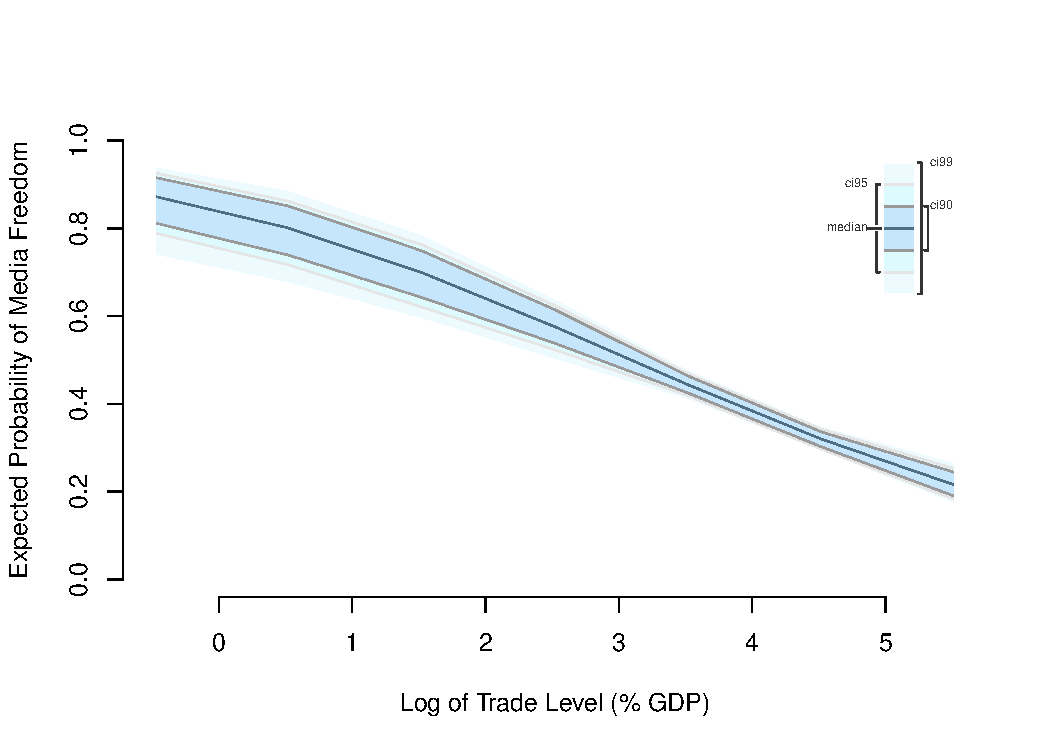
\includegraphics[width=\maxwidth]{figures/Trade_Effect_Plot1} 

}




{\centering 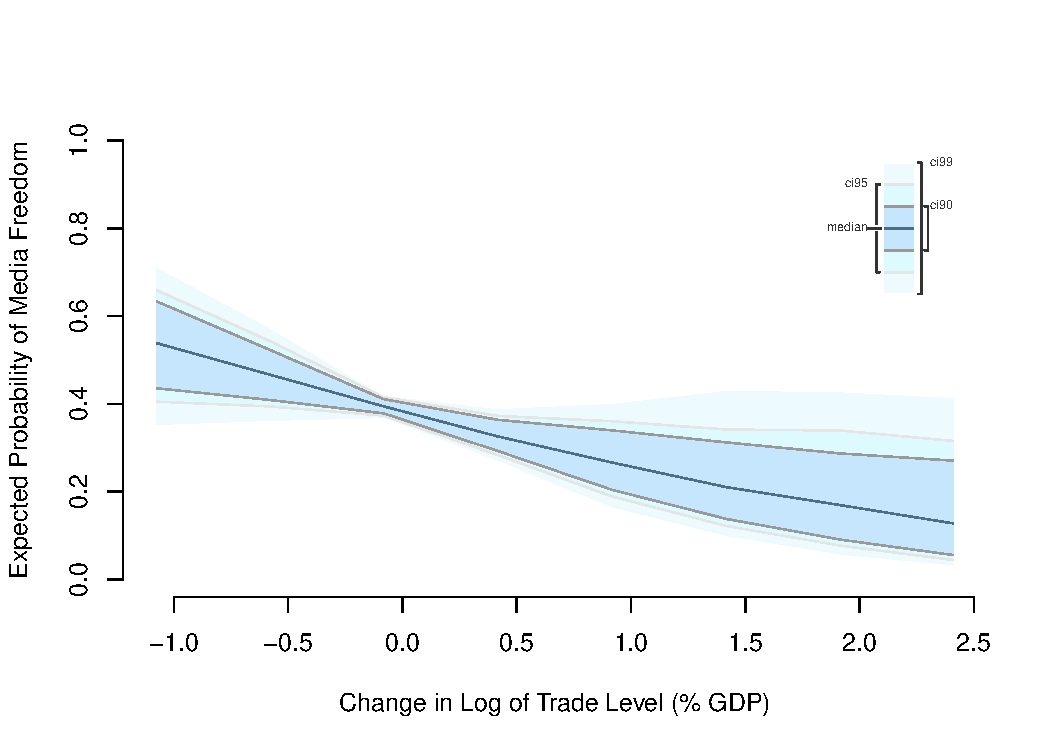
\includegraphics[width=\maxwidth]{figures/Trade_Effect_Plot2} 

}



\end{knitrout}
  \end{center}
    \begin{singlespace}
        {\scriptsize{}}
    \end{singlespace}
\end{figure}
\clearpage
}

As logit estimates are not conveniently interpretable, the top half of Figure 2 illustrates the long-run expected probability of observing media freedom in $country_{it}$ given different levels of international trade.\footnote{All discussion of predicted probabilities are based on 1000 simulations of the model. The simulations were conducted in R with the package \emph{Zelig} \parencite*{ZeligEveryonesSt:2009ts}.} The expected probability of observing media freedom in a country completely closed to international trade, with mean values on all other variables in the model, is 0.84. Increasing international trade from zero to the mean of 4.06 would be expected to decrease the probability of media freedom by \ensuremath{-0.46} to 0.38.

The bottom half of Figure 2 illustrates how the expected probability of observing media freedom in $country_{it}$ is expected to change in the short-run in response to yearly changes in level of international trade. The expected probability of observing media freedom in a country with a mean trade level of 4.06 but zero change in trade is 0.38. A yearly increase in logged trade of 0.15, a yearly change of trade one standard deviation above the mean yearly change, would be expected to decrease the probability of media freedom by \ensuremath{-0.02} to 0.36.


% 
% \afterpage{
% \begin{figure}[t]
%     \caption{Simulated Effect of FPI Stock on Expected Probability of Media Freedom}
%     \label{absolute}
%     \begin{center}
% <<FPI_Effect_Plot, fig.align='center', fig.height=5, cache=FALSE>>=
% source("/Users/justin/Dropbox/gh_projects/globalization_media_freedom/analyses/fpi_effect_plot.R")
% @
%   \end{center}
%     \begin{singlespace}
%         {\scriptsize{Expected values from 1000 simulations of Model 3 in Table 1.}}
%     \end{singlespace}
% \end{figure}
% \clearpage
% }
% 
% The top half of Figure 3 plots the expected probability of observing media freedom in $country_{it}$ given increases in FPI stocks. The expected probability of observing media freedom given zero FPI stock and all other variables held constant at their mean is mean(unlist(s.out.fpi$qi[1])). An increase in FPI stock from zero to the mean value of (mean(df$lfpistock2)), would be expected to increase the probability of media freedom by mean(s.out.fpi$qi$fd) to mean(unlist(s.out.fpi$qi[2])).
% 
% The bottom half of Figure 3 plots the expected probability of observing media freedom in $country_{it}$ in the short-run due to yearly changes in FPI stock (FPI inflows). The expected probability of observing media freedom given zero FPI inflow and all other variables held constant at their mean is mean(unlist(s.out.fpi.change$qi[1])). The mean FPI inflow per year, (mean(df$dfpistock2)), increases the probability of media freedom by mean(s.out.fpi.change$qi$fd) to mean(unlist(s.out.fpi.change$qi[2])).

\subsection{Robustness}

This section examines the robustness of the regression models in multiple ways. First, I consider the possibility that the model results presented above may be disproportionately driven by regression outliers or outliers in trade openness. Second, I use Bayesian Model Averaging to assess the sensitivity of the above results to model selection. Third, I check for evidence of endogeneity and reverse-causality in particular. Fourth, I use genetic matching to mitigate against bias due to non-random assignment of trade openness and I calculate how sensitive my estimates are to a potential omitted variable.

\subsubsection{Outliers}

Considering Bonferonni-adjusted p-values for the largest Studentized residual in Model 5 using a normal distribution test, we fail to reject the null hypothesis that there are no outliers.\footnote{Numerical results are not reported for the sake of brevity but are reproducible from the replication repository.} While there is no evidence of problematic regression outliers, the right-skew of trade openness raises the possibility that the negative relationship between trade openness and media freedom is disproportionately driven by cases of extreme trade openness and does not accurately reflect most cases. The main regression results already mitigate this possibility by using the log of trade openness, which significantly compresses its distribution. Yet even the log of trade openness contains 107 observations greater than 1.5 times the interquartile range and the first differences of logged trade openness contain 340 such observations. Removing these observations from Model 6 decreases the magnitude of the coefficient (.98) but it remains signed as expected, still larger than the estimate of Model 5, and statistically significant at the 99\% confidence level.\footnote{For full model results, see Table 5 in Supplementary Information.} In summary, there appears little reason to believe that the model results presented here are artifacts of regression outliers or extreme cases of trade openness.

\subsubsection{Bayesian Model Averaging}

An idiosyncratic search for optimal model specifications can lead to publication bias (as researchers will tend to prefer models that confirm their hypotheses), decreased efficiency (if researchers include too many unnecessary control variables), and incomplete representations of model uncertainty and sensitivity \parencite[2]{Montgomery:2010fc}. One technique for gauging the robustness of particular independent variables against model uncertainty is Bayesian Model Averaging (BMA), which estimates all possible models from a set of variables and calculates posterior probabilities for all possible coefficients and models \parencite[4]{Montgomery:2010fc}. BMA allows analysts to identify the most likely models given data, and then the probability particular independent variables will appear in the most likely models.

To check the robustness of the estimates reported above, this subsection reports results from a BMA analysis of the entire model space of Model 6. Because this article focuses on disentangling the effects of economic globalization on media freedom, the analysis includes the full battery of economic globalization indicators, despite the relatively limited availability of FPI data. In a subsequent analysis discussed in the appendix, I conduct BMA on the significantly more data-rich model space of Model 5. The BMA analysis uses uniform priors for all independent variables.\footnote{The analysis was conducted using the \emph{bic.glm()} function in the R package \emph{BMA} \parencite{BMABayesianModel:us}.}

\afterpage{
\begin{figure}[t]
    \caption{BMA: Occurrence of variables in most likely models}
    \label{absolute}
    \begin{center}
\begin{knitrout}
\definecolor{shadecolor}{rgb}{0.969, 0.969, 0.969}\color{fgcolor}

{\centering 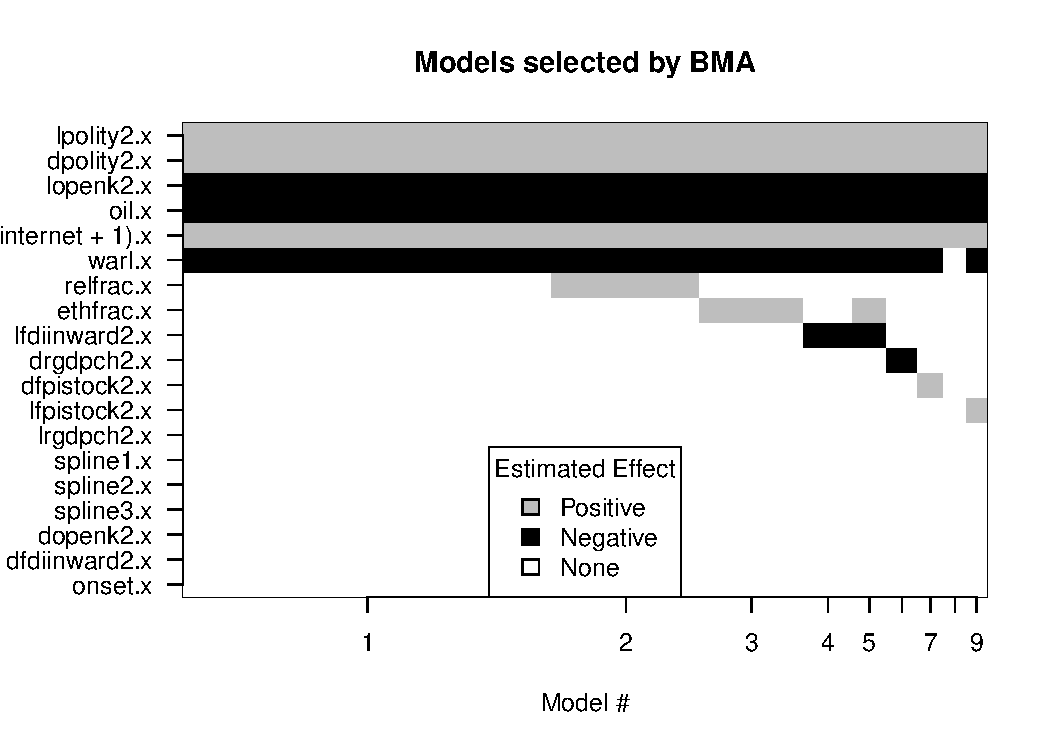
\includegraphics[width=\maxwidth]{figures/BMA_Plot} 

}



\end{knitrout}
  \end{center}
    \begin{singlespace}
        {\scriptsize{}}
    \end{singlespace}
\end{figure}
\clearpage
}

\afterpage{
\begin{figure}[t]
    \caption{BMA: Probabilities of inclusion}
    \label{absolute}
    \begin{center}
\begin{knitrout}
\definecolor{shadecolor}{rgb}{0.969, 0.969, 0.969}\color{fgcolor}

{\centering 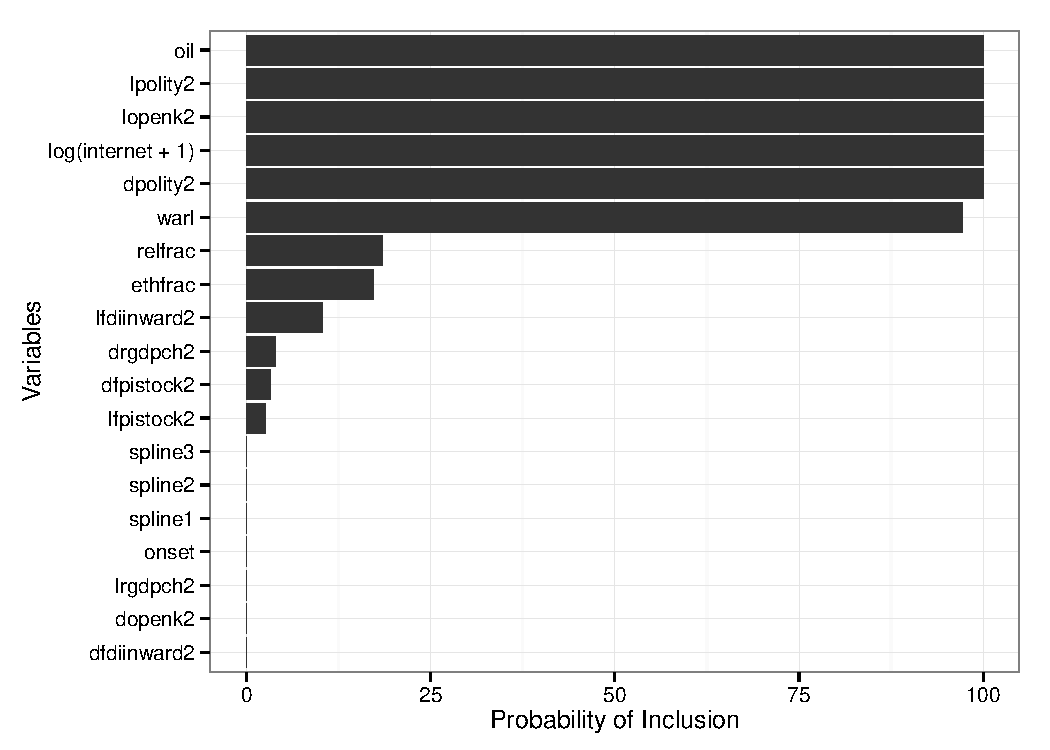
\includegraphics[width=\maxwidth]{figures/BMA_Plot_Inclusions} 

}



\end{knitrout}
  \end{center}
    \begin{singlespace}
        {\scriptsize{}}
    \end{singlespace}
\end{figure}
\clearpage
}

The results suggest that levels of trade openness have a robust negative effect on media freedom. Lagged levels of trade openness have a negative and statistically significant association with media freedom in 100\% of the 9 model specifications with the highest posterior probabilities. While levels of FDI have a negative association with media freedom in some models, the probability of this association appearing in the 9 most likely models is only .13. Stocks and flows of FPI are positively and significantly associated with media freedom, but only with .26 and .33 probabilities, respectively.

\subsubsection{Endogeneity}

As democracy affects trade levels \parencite{Milner:2005ci}, it is possible that changes in media freedom affect trade levels for the same reason, as pro-trade or anti-trade domestic groups politically empowered by free media shape trade policy toward greater or less openness. If media freedom affects trade policy, then the regression estimates in Table 1 would be incorrect. I consider this possibility in two ways. First, if reverse causality is present and creating bias in the regression estimates, then some regressors should be correlated with the error term (endogeneity). Diagnosing this question manually reveals that the correlation coefficient for trade openness and the residuals is 0 and does not exceed 0.08 for all other independent variables in Model 5, providing no obvious evidence of endogeneity. Second, I estimate a series of ordinary least-squares (OLS) regressions modeling the trade variable as a function of lagged values of media freedom, including fixed effects for year and country.\footnote{See Table 5 in Supplementary Information for full results.} A simple model with no controls other than fixed effects and a second model controlling additionally for levels and changes of democracy and economic growth both suggest that lagged values of media freedom have a positive and significant effect on trade levels. A third model controlling for lagged levels of trade openness suggests media freedom has no statistically distinguishable association with level of trade openness. Thus, the only evidence of reverse causality suggests that media freedom could possibly have a positive effect on trade openness. This is not problematic for the central argument that trade has a negative effect on media freedom because the direction of the effect would, if anything, bias the estimates in Table 1 upward. That is, to the degree media freedom increases trade, this would not lead to spurious evidence in favor the central argument but would rather lead to underestimating the negative effect of trade on media freedom. Given these two checks, the estimated negative effect of trade on media freedom appears robust to the threat of reverse causality.

\subsubsection{Matching and Sensitivity Analysis}



Another problem for regression analysis of observational data is that if the propensity for units of analysis to realize certain values on an independent variable of interest (in this case, trade openness) is shaped by some other variable, estimates for that independent variable will be biased. To mitigate the risks of this problem, I use a genetic matching search algorithm to automatically create a subset of the original sample which is optimally balanced with respect to the other covariates \parencites{Diamond:2012jo}{Sekhon:2008wd}. If any of the observed covariates shape the propensity of a unit to realize higher levels of trade openness, which would lead to biased estimates of trade's effect, the algorithm identifies the weights which need to be applied to each covariate to create matched pairs of treatment and control units to optimize balance in the propensity to be treated. After this procedure, the average treatment effect for the treated will approximate that which would be inferred from a randomized experiment, assuming of course that there is no unobserved factor shaping the propensity to be treated omitted from the matching procedures. While the risk of omitted variables is impossible to rule out, it is possible to quantify the sensitivity of matching estimates to a hypothetical, unobserved source of bias. Thus, I also report sensitivity bounds following the procedures developed by Rosenbaum \parencite*{Rosenbaum:1988fl}, in order to state how large an unobserved source of bias would have to be to account for the estimated treatment effect. For this analysis, I used the full set of economic openness variables (Model 6) because, if it is plausible that FDI and FPI are associated with a country's propensity to realize trade openness, it would be necessary to estimate the effect of trade from countries balanced with respect to these variables as well as the control variables.

The average treatment effect from a logged trade level greater than the mean is \ensuremath{-0.08}, with a standard error of 0.02 and a p-value of 0.0002. The matching estimate is signed consistently with the findings of the previous sections and statistically significant at the 99\% level. Calculation of Rosenbaum bounds suggests that, for this effect to become statistically insignificant at the 95\% confidence level, the odds of differential assignment due to an unobserved factor would have to be about 2.26.\footnote{Rosenbaum bounds for a binary dependent variable are calculated using the \emph{binarysens()} function in the R package \emph{rbounds} \parencite{rboundsPerformRos:2014vj}.} Thus, it is unlikely that the negative relationship between trade openness and media freedom estimated in the main models is merely an artifact of non-random assignment into the treatment of trade openness.



% 
% \afterpage{
% <<Interesting_Cases, results='asis', cache=FALSE>>=
% source("/Users/justin/Dropbox/gh_projects/globalization_media_freedom/analyses/explained_cases.R")
% require(stargazer)
% stargazer(model3.cases,
%           title="Cases Incorrectly Classified by Democracy and Domestic Economy but
%                       Correctly Classified by Adding Globalization Predictors",
%           style = "apsr",
%           summary=FALSE,
%           digit.separator=""
%                       )
% @
% \clearpage
% }
% 
% \afterpage{
% \begin{figure}[t]
%     \caption{Cases Unexplained by Democracy and Domestic Economy: Haiti, Malawi, Armenia, and Ukraine}
%     \label{absolute}
%     \begin{center}
% <<Explained_Cases_Plots, fig.align='center', cache=FALSE>>=
% source("/Users/justin/Dropbox/gh_projects/globalization_media_freedom/analyses/explained_cases_plots.R")
% grid.arrange(haiti_malawi_plots, ukraine_armenia_plots)
% @
% \end{center}
%     \begin{singlespace}
%         {\scriptsize{Grey shading indicates periods of media repression (\emph{Media Freedom} = 0).
%         International economic variables are measured as shares of GDP.
%         GDP per capita is divided by 100.
%         Freedom House Freedom of the Press Scores are on a 0-100 scale.}}
%     \end{singlespace}
% \end{figure}
% \clearpage
% }




\section{Qualitative Within-Case Analysis}

Next, I provide two brief case studies of Argentina and Mexico to assess qualitatively whether we can observe implications of trade liberalization generating pressures toward media repression.

\afterpage{
\begin{figure}[t]
    \caption{Globalization and Media Freedom in Argentina and Mexico, 1980-2003}
    \label{absolute}
    \begin{center}
\begin{knitrout}
\definecolor{shadecolor}{rgb}{0.969, 0.969, 0.969}\color{fgcolor}

{\centering 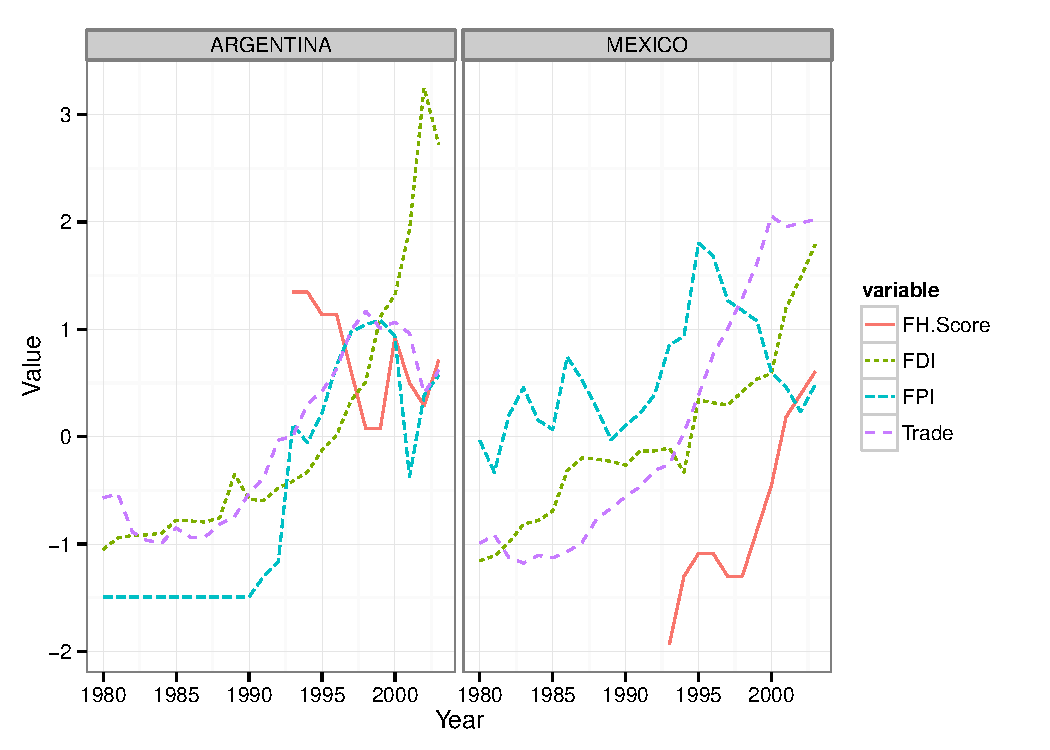
\includegraphics[width=\maxwidth]{figures/Case_Studies_Plots} 

}



\end{knitrout}
  \end{center}
    \begin{singlespace}
        {\scriptsize{Values are scaled to represent standard deviations from a mean of zero. Economic variables are measured as shares of GDP, as discussed in the main text. Freedom House Freedom of the Press Scores are on a 0-100 scale.}}
    \end{singlespace}
\end{figure}
\clearpage
}

\subsection{Argentina}

Immediately upon inauguration as President in 1989, Carlos Menem announced a package of neoliberal economic reforms which include liberalization of international trade and capital flows, as well as privatizations and spending cuts \parencites[189]{Tommasi:1995wx}{Borner:2002cp}. In the beginning of 1989, the average tariff rate is 39\% (a maximum import tariff was 50\% with a tariff surcharge of 15\% on all imports). By the end of 1989, the maximum tariff is 35\% and the average tariff rate falls to 12\%. In 1990, all import licensing requirements are abolished and tariffs are reduced across-the-board to 21\%. By 1995, the average unweighted tariff is 10.5\% and non-tariff barriers as well as export restrictions are removed. Exemptions were made for IT, domestic appliances, and autos. As a result, imports increased from \$4.1 billion in 1990 to \$21.6 billion in 1994, while exports increased from \$3.7 billion to \$20.1 billion at the same time \parencite[7]{Beker:2011vq}.

As import competition put pressure on previously protected firms, there was a 30\% decrease in manufacturing employment between 1992 and 1996. In those industries where import penetration increased the most, wage inequality also widened during this period. Argentina's Gini coefficient for income inequality, one of the lowest in Latin America at the time, increased from 40.0 in 1991 to 47.4 by 1998 \parencites[505]{Galiani:2003fr}[11]{Beker:2011vq}.

Argentina will join the Mercosur customs union in 1991 and sign a trade agreement with the United States in 1994. The reform package largely succeeded in taming inflation rates and growing the economy. The inflation rate shrinks from 5\% in 1989 to .16\% by 1996 and gross domestic product grows by 40\% between 1990 and 1994 \parencite[4]{Beker:2011vq}. The IMF, World Bank, and the US government saw Argentina as a model student in this period \parencites[142]{Cavallo:2004bf}{Cavallo:2004ta}[167]{Klein:2002vg} and is frequently cited in leading global publications such as \emph{Time International} as a poster child for how neoliberal economic reforms should be implemented (\emph{Time International} \cite*{:3GmqDB3y}, as cited in \cites[194]{Echegaray:2001tf}{MarcusDelgado:2003gn}{Silverstein:2002wm}).

Although the reform package succeeds in taming Argentina's hyperinflation and creating economic growth, the most immediate and direct effect of trade liberalization was an increase in unemployment, especially among the workforce employed in previously protected, labor-intensive industries \parencite[10]{Beker:2011vq}. Additionally, trade liberalization reduced the income of small-scale producers who could not compete with cheap imports \parencite{eckstein2001power}. Although trade liberalization is costly to the sizable constituencies of unskilled industrial workers and rural campesinos, the government provides little public support for dislocated workers--reducing rather than increasing public spending--until the government develops a targeted income-assistance program during the currency crisis of 2001. This lack of government responsiveness between 1990 and 2001 is puzzling given the longstanding expectation that governments, and especially democratic regimes, must compensate domestic losers from liberalization in order to sustain a sufficient political coalition in favor of liberalization. This expectation should be especially strong for democratic governments, yet, despite the absence of government compensation, Argentina sees relatively little domestic conflict around trade liberalization. In fact, there are fewer strikes, strikers, and days lost to strikes than under Alfonsin \parencite{eckstein2001power}. Yet, dissent against liberalization was an observable current in public discourse in the years before Menem's repressive media regulations. It is worth noting that some of the media scandals related to government corruption were themselves linked to international economic openness. For instance, the aggressive Argentine daily Pagina/12, whose journalists were frequent targets of violence, sparked a scandal when they reported on the Menem administration requiring ``substantial payment'' from the meatpacking firm Swift-Armour before they were allowed to import machinery into the country. Another highly publicized revelation involved the complicity of government officials in an international drug-laundering network \parencite{Waisbord:1994kq}. Most notably in road blockages organized by protesting farmers in 1991 and 1993, unfair international competition was a recurring point of dissent \parencites{McCullough:1991cs}{Ferber:1993fb}.

If the Menem regime neglected to make provisions for its harmed constituencies, how was it able to enact and sustain dramatic trade and capital liberalization in a formally democratic setting? The theory presented here expects that the Menem government is likely to repress the media in order to silence domestic opposition to liberalization while maintaining a formally democratic front. Consistent with the theory, the quantitative data reveal that after a long and stable period of stable economic openness and media freedom under Alfonsin, media freedom is volatile immediately after Menem's liberalization begins until it is stably repressed by 2005. According to a report Agresiones a La Prensa 1991-1994 published by the Asociacion Madres de Plaza de Mayo, around 452 acts of aggression were committed against the press between 1991 and 1994 (Delgado \cite*{Delgado:1995tr}, as cited in \cite[247]{Park:2002io}). Acts of aggression refer to “murder, death threats, bombings, bomb threats, intimidation, physical violence, violent threats, and termination of broadcasts.” If one were to count acts of excluding media from access to the government and public name-calling of the media by the government, the figure would be 546. Although not perpetrated directly by the state, during this period there were many acts of violence against investigative journalists critical of the Menem regime, acts which the government denounced but treated with impunity \parencite{Long:1993wb}. The Menem family's most direct actions against media freedom were cuts to state advertising in Pagina/12 \parencite[27]{Waisbord:1994kq}, 11 lawsuits against journalists under the pretense of criminal defamation \parencite{McCullough:1991cs}, proposals to increase libel and defamation sentencing, and a proposal to require media outlets to purchase prohibitively expensive libel insurance \parencite{Sims:kgMPqAHd}.

\subsection{Mexico}

As in the case of Argentina, Mexico's trade liberalization in the 1990s was part of a larger national project of neoliberal economic reform. Well before signing the North American Free Trade Agreement (NAFTA) with the United States and Canada in 1994, Mexico unilaterally lowered tarrifs from an average of 25\% in 1985 to 13\% by 1993 \parencite{McDaniel:2003kw}.

Concurrent with unilateral trade liberalization and NAFTA, and as in the case of Argentina under Menem, the Mexican government also privatized many state-owned enterprises and eliminated many state subsidies and price controls originally intended to support small farmers. Most subsidies for corn and wheat producers and retail food price controls were eliminatd by 1991 \parencite[295]{Hufbauer:2005vh}. In 1999, the Mexican government abolished CONASUPO, the state agency which bought staple crops at guaranteed prices and redistributed them to consumers \parencite[12]{Villareal:2010vk}.

After NAFTA, US imports from the US increased from \$50.8 in 1994 to 100.4 billion in 2000 \parencite[10]{Villareal:2010vk}. As in the case of Argentina, trade liberalization through the 1990s hurt small farmers and non-skilled manufacturing, as agricultural employment decreased from 8.1 million in 1993 to 6.8 million jobs in 2003, and value added decreased from \$32 billion to about \$25 billion in the same period.\parencites[289]{Hufbauer:2005vh}[14]{Villareal:2010vk}.

Also as in Argentina, increasing trade liberalization in Mexico led to increased wage inequality between skilled and non-skilled labor. In 1988, the real average wage level of skilled Mexican workers in the manufacturing sector was 225\% that of non-skilled workers. In 1996, it was about 290\% that of non-skilled workers, stabilizing until 2000 \parencite[9]{Villareal:2010vk}.

To support the transition into NAFTA, the government enacted the Programa de Apoyos Directos para el Campo (Program of Direct Support for the Countryside or “Procampo”), which provided farmers with direct, hectare-based income support. However, in part due to austerity following the peso crisis, total expenditure on Procampo decreased from \$1.4 billion to \$1 billion \parencite[295]{Hufbauer:2005vh}, despite the price of corn in Mexico falling from \$4.84 per bushel in 1993 to \$3.65 in 1997 \parencite[12]{Villareal:2010vk}, the total number of supported farmers decreased from 3.29 million to 2.95 million, between 1994 and 1998 \parencite[295]{Hufbauer:2005vh}.

On the day NAFTA went into effect in January 1994, the Ejército Zapatista de Liberación Nacional (EZLN) launched an armed uprising in one of Chiapas, one of Mexico's southernmost states. On that very first day of the uprising, EZLN spokesperson Subcomandante Marcos declared NAFTA to be “nothing more than a death sentence to the indigenous ethnicities of Mexico” and their uprising to be understood as a response “to the decree of death that the Free Trade Agreement gives them” (\emph{La Journada} 1994, as cited in \cite[216]{Hayden:2009uy}.

Although Procampo helped gain support for NAFTA, immediately there was popular discontent, such as in the Barzón Farmers movement in Zacatecas, regarding several inadequacies of the program, including payments not being made \parencite[173]{Williams:2001ux}. From 1993 to 1995, the Barzon movement sought and received much favorable attention in the print media, where reporters were not under great pressure to suppress reports \parencite[187]{Williams:2001ux}.

Neoliberal economic reforms, including increasing trade openness, somewhat surprisingly in light of our expectations although not exactly contradicting them, led to a relative opening of the domestic media \parencite{lawson2002building}. Between 1991 and 1993, in addition to pursuing NAFTA as his administration's top priority, Salinas' cuts to government spending included cutting the quid pro quo's which underwrote the traditional regime of media control. He specifically ended the system of paying for reporters accomodations on presidential trips, prohibited the distribution of bribes within the presidential palace, reduced the government advertising in which typically functioned as bribes for keeping media in line, ended tax deferments and credits to media, and stopped allowing media outlets to pay their Social Security taxes in advertisements. Privatization of state-owned enterprises also had the effect of reducing the media's dependence on government advertising revenues. The greater scrutiny from American and Canadian media relaxed the domestic media environment for domestic journalists, as it was easier for domestic journalists to report on topics that the foreign press were already reporting on outside any control from the Mexican government. Additionally, greater access to foreign inputs also freed the Mexican media from an important source of government leverage, in particular its traditional monopoly on the import of newsprint, providing further room for the Mexican media to take risks. As independent media outlets were gaining financial independence through market competition, at the same time the neoliberal state was relinquishing its traditional levers of control, led to a independence of the Mexican media increased significantly \parencite[76,89]{lawson2002building}.

The international spotlight from the NAFTA negotiations also forced Salinas to cultivate a more positive image on human rights, for instance, when he established the National Commission for Human Rights \parencite[107]{Dominguez:2009wd}. Additionally, because neoliberal economic reforms actually led to an opening of the media which the state could not control, Salinas and after him Ernesto Zedillo moved away from traditional tactics of media repression in favor of more modern techniques of “news management” and public relations, such as controlling information by only providing access to friendly reporters. For instance, in a 1990 press conference Salinas explicitly excluded several independent media outlets and only permitted the most reliable pro-government journalists. Later in 1996, the Interior Ministry for the first time created an explicit “blacklist” of journalists who government officials were supposed to not engage \parencite[39]{lawson2002building}.

Newspaper circulation is limited in Mexico, whereas television broadcasting dominated by Televisa is the main source of information, so it was dominated by pro-NAFTA, pro-government ideology \parencite{Hellman:1993wa}. They also used it for extensive foreign media campaigning. While building support for NAFTA, Salinas used media and PR tools extensively, including efforts to persuade Mexican-Americans and US investors to support NAFTA in the United States \parencite{Morris:2001iy}. This was the first time the Mexican government used advertising and lobbying in its foreign relations \parencite{Chabat:1997wj}. One of the most commented advertisements urged US business to look to Mexico as a place where they can hire workers for a dollar an hour \parencites[105]{center1993trading}[45]{Chabat:1997wj}.

This narrative reveals dynamics which are unexpected and in a crucial sense antithetical to our theory, for they reveal how economic liberalization may induce greater media freedom by increasing competition and growth. Yet, Salinas in particular was convinced that he had to protect the government's image to succeed in his foreign economic policies \parencite[107]{Dominguez:2009wd}. Although economic reforms made certain kinds of repression impracticable, under Salinas and then Zedillo the Mexican government engaged in specific acts to exclude the press from reporting on politically sensitive issues. Lawson observes plainly that Salinas was historically Mexico's “undisputed master of image management” \parencite[39]{lawson2002building}. Additionally, the editor of Mexico's Monitor, José Gutiérrez-Vivó, affirmed in 1996 that “Salinas was the president who was hardest on the media. He was the one who sought the most control over the media” \parencite[39]{lawson2002building}. After NAFTA passes, intimidation and direct violence against journalists at the hands of the state can still be observed, as when the state expropriates the property of critical editors \parencite{OrmeJr:1997da}. In fact, despite a de facto opening of the media due to financial independence and the neoliberal withdrawal of the state from private enterprise, federal state-media relations changed little until Zedillo and even his adminstration engaged in repressive tactics such as arresting the publisher of El Universal for tax-related reasons in 1996. Finally, physical assault against journalists increased throughout the period of Mexican media's opening from 1980 to the middle of the 1990s \parencite[81]{lawson2002building}, which was also a period of dramatic trade opening. Most of the physical assaults were not carried out by the government, but they were largely treated with impunity by the government.

Thus, in the process of trade liberalization, Mexican state officials actively seek greater control over the media as much as they can, despite the effect of increased competition unleashing an increasingly independent media. Both Salinas and Zedillo employed a variety of tactics ranging from traditional repression to modern “news management” in order to control their image in the media during a period of rapid trade liberalization. Salinas in particular, the earliest and most aggressive proponent of economic liberalization in the late 1980s and early 1990s, tried more than anyone else to control the media.

\section{Conclusion}

More trade-open countries are more likely to repress the media because, while the distributive conflicts generated by economic liberalization tempt national policymakers to repress the media, international trade is uniquely permissive of this repressive tendency, whereas international capital investment generates countervailing incentives against repression. This article provides a mix of quantitative and qualitative evidence suggesting that a country undergoing trade liberalization in particular is more likely to have a repressive media environment, even after controlling for previously well-established drivers of media freedom such as regime type, income levels, and economic growth. Several statistical models and robustness checks including Bayesian Model Averaging and genetic matching show that, unique among the components of globalization considered here, trade levels have a robust negative association with media freedom. On the other hand, while there is some limited evidence that FDI has a negative association with media freedom in the long-run and FPI has a positive association with media freedom in the short- and long-run, these findings were found to be highly sensitive to model selection. Finally, qualitative process-tracing on cases from Argentina and Mexico in the early 1990s, selected as relatively hard cases of consolidating democracies which for that reason strongly predict media freedom, each provide some illustration of the mechanism relating trade openness to media repression. The regimes of Carlos Menem in Argentina and Carlos Salinas in Mexico both saw media freedom decrease at moments illustrative of the theory.

The implications of this article are important for several reasons. First, this article provides the first systematic, large-N statistical inquiry into the relationship between economic globalization and media freedom. In particular, the article places into scholarly view the surprisingly under-reported empirical anomaly that media freedom historically has a weakly negative association with trade openness, despite having a positive association with general indices of economic globalization and despite the conventional wisdom that economic openness is generally associated with domestic political openness. The robust documentation of this stylized fact poses a unique puzzle which will be of interest to scholars of the globalization-democracy nexus and IPE/CPE more generally because it represents a striking exception to the widespread expectation that economic openness will typically be associated with domestic political openness. Second, the theoretical rationale presented to account for this stylized fact contributes a novel theoretical insight to current research on the globalization-democracy nexus and on the mechanisms of anocratic government because it highlights a specific causal pathway whereby an international economic variable can generate unique pressures toward repressive state behavior, even within relatively democratic countries. Finally,
researchers of state-media relations (as well as activists and policy-makers interested in promoting media freedom) will be interested in the findings presented here because they highlight a new causal path, hardly if at all understood in current political media research, affecting the probability a state will liberalize or repress the media.


\clearpage

\section{Supplementary Information}


% Table created by stargazer v.5.1 by Marek Hlavac, Harvard University. E-mail: hlavac at fas.harvard.edu
% Date and time: Wed, Jan 14, 2015 - 18:37:19
\begin{table}[!htbp] \centering 
  \caption{Summary Statistics} 
  \label{} 
\small 
\begin{tabular}{@{\extracolsep{5pt}}lccccc} 
\\[-1.8ex]\hline 
\hline \\[-1.8ex] 
Statistic & \multicolumn{1}{c}{N} & \multicolumn{1}{c}{Mean} & \multicolumn{1}{c}{St. Dev.} & \multicolumn{1}{c}{Min} & \multicolumn{1}{c}{Max} \\ 
\hline \\[-1.8ex] 
fp & 7,849 & 0.450 & 0.500 & 0 & 1 \\ 
year & 7,858 & 1,987.000 & 15.000 & 1,960 & 2,011 \\ 
lpolity2 & 7,273 & 0.470 & 7.500 & $-$10 & 10 \\ 
dpolity2 & 7,261 & 0.079 & 1.700 & $-$18 & 16 \\ 
lrgdpch & 7,330 & 9,655.000 & 20,327.000 & 400.000 & 632,240.000 \\ 
drgdpch2 & 7,324 & 0.015 & 0.097 & $-$1.500 & 1.100 \\ 
lopenk & 7,346 & 70.000 & 46.000 & 0.310 & 444.000 \\ 
dopenk2 & 7,327 & 0.012 & 0.150 & $-$1.200 & 2.700 \\ 
lfdiinward & 5,789 & 20.000 & 45.000 & 0.000 & 1,165.000 \\ 
dfdiinward2 & 5,788 & 0.069 & 0.240 & $-$2.100 & 2.200 \\ 
lfpistock2 & 3,009 & 2.000 & 1.500 & 0.000 & 8.700 \\ 
dfpistock & 2,922 & 1.600 & 52.000 & $-$1,678.000 & 1,707.000 \\ 
oil & 7,732 & 0.150 & 0.350 & 0 & 1 \\ 
internet & 7,271 & 0.730 & 1.300 & 0.000 & 4.600 \\ 
ethfrac & 7,213 & 0.400 & 0.280 & 0.001 & 0.930 \\ 
relfrac & 7,213 & 0.380 & 0.220 & 0.000 & 0.780 \\ 
warl & 7,393 & 0.150 & 0.350 & 0 & 1 \\ 
onset & 7,393 & 0.014 & 0.120 & 0 & 1 \\ 
\hline \\[-1.8ex] 
\end{tabular} 
\end{table} 


\afterpage{

% Table created by stargazer v.5.1 by Marek Hlavac, Harvard University. E-mail: hlavac at fas.harvard.edu
% Date and time: Wed, Jan 14, 2015 - 18:37:20
\begin{table}[!htbp] \centering 
  \caption{List of countries included in the statistical analyses} 
  \label{} 
\scriptsize 
\begin{tabular}{@{\extracolsep{5pt}} ccc} 
\\[-1.8ex]\hline 
\hline \\[-1.8ex] 
ALBANIA & ALGERIA & ANGOLA \\ 
ARGENTINA & ARMENIA & AUSTRALIA \\ 
AUSTRIA & AZERBAIJAN & BAHRAIN \\ 
BANGLADESH & BELARUS & BELGIUM \\ 
BENIN & BOLIVIA & BOTSWANA \\ 
BRAZIL & BULGARIA & BURKINA FASO \\ 
BURUNDI & CANADA & CENTRAL AFRICAN REPUBLIC \\ 
CHILE & CHINA & COLOMBIA \\ 
CONGO & COSTA RICA & COTE D'IVOIRE \\ 
CROATIA & CYPRUS & CZECH REPUBLIC \\ 
CZECHOSLOVAKIA & DENMARK & DOMINICAN REPUBLIC \\ 
ECUADOR & EGYPT & EL SALVADOR \\ 
ERITREA & ESTONIA & ETHIOPIA \\ 
FIJI & FINLAND & FRANCE \\ 
GAMBIA & GEORGIA & GERMANY \\ 
GHANA & GREECE & GUATEMALA \\ 
GUINEA & GUINEA-BISSAU & GUYANA \\ 
HONDURAS & HUNGARY & INDIA \\ 
INDONESIA & IRAN & IRAQ \\ 
IRELAND & ISRAEL & ITALY \\ 
JAMAICA & JAPAN & JORDAN \\ 
KAZAKHSTAN & KENYA & KOREA \\ 
KUWAIT & KYRGYZSTAN & LATVIA \\ 
LIBYAN ARAB JAMAHIRIYA & LITHUANIA & MACEDONIA \\ 
MALAWI & MALAYSIA & MALI \\ 
MAURITANIA & MAURITIUS & MEXICO \\ 
MOLDOVA & MONGOLIA & MOROCCO \\ 
MOZAMBIQUE & NAMIBIA & NEPAL \\ 
NETHERLANDS & NEW ZEALAND & NICARAGUA \\ 
NIGER & NIGERIA & NORWAY \\ 
PAKISTAN & PANAMA & PARAGUAY \\ 
PERU & PHILIPPINES & POLAND \\ 
PORTUGAL & ROMANIA & RUSSIAN FEDERATION \\ 
RWANDA & SAUDI ARABIA & SENEGAL \\ 
SIERRA LEONE & SINGAPORE & SLOVAKIA \\ 
SLOVENIA & SOMALIA & SOUTH AFRICA \\ 
SPAIN & SRI LANKA & SUDAN \\ 
SWAZILAND & SWEDEN & SWITZERLAND \\ 
TANZANIA & THAILAND & TOGO \\ 
TUNISIA & TURKEY & UGANDA \\ 
UKRAINE & UNITED KINGDOM & UNITED STATES \\ 
URUGUAY & VENEZUELA & VIETNAM \\ 
YUGOSLAVIA & ZAMBIA & ALBANIA \\ 
\hline \\[-1.8ex] 
\end{tabular} 
\end{table} 

\clearpage
}

\afterpage{

% Table created by stargazer v.5.1 by Marek Hlavac, Harvard University. E-mail: hlavac at fas.harvard.edu
% Date and time: Wed, Jan 14, 2015 - 18:37:25
\begin{table}[!htbp] \centering 
  \caption{Model 6 of Table 1 with trade outliers removed} 
  \label{} 
\footnotesize 
\begin{tabular}{@{\extracolsep{5pt}}lc} 
\\[-1.8ex]\hline \\[-1.8ex] 
\hline \\[-1.8ex] 
 Democracy$_{t-1}$ & 5.00$^{***}$ \\ 
  & (0.16) \\ 
  $\Delta$Democracy & 0.61$^{***}$ \\ 
  & (0.08) \\ 
  GDP per capita$_{t-1}$ & 0.13 \\ 
  & (0.17) \\ 
  $\Delta$GDP per capita & 0.08 \\ 
  & (0.13) \\ 
  Spline 1 & $-$0.08 \\ 
  & (0.47) \\ 
  Spline 2 & $-$0.88 \\ 
  & (1.70) \\ 
  Spline 3 & $-$0.47 \\ 
  & (0.39) \\ 
  Trade$_{t-1}$ & $-$0.98$^{***}$ \\ 
  & (0.15) \\ 
  $\Delta$Trade & $-$0.20 \\ 
  & (0.17) \\ 
  FDI$_{t-1}$ & 0.27$^{*}$ \\ 
  & (0.14) \\ 
  $\Delta$FDI & 0.15 \\ 
  & (0.11) \\ 
  FPI$_{t-1}$ & $-$0.15 \\ 
  & (0.16) \\ 
  $\Delta$FPI & 0.93$^{***}$ \\ 
  & (0.23) \\ 
  Oil$_{t-1}$ & 0.48$^{***}$ \\ 
  & (0.12) \\ 
  Internet$_{t-1}$ & 0.31$^{***}$ \\ 
  & (0.11) \\ 
  Ethnic Frac.$_{t-1}$ & $-$1.70$^{***}$ \\ 
  & (0.42) \\ 
  Religious Frac.$_{t-1}$ & $-$0.95$^{***}$ \\ 
  & (0.13) \\ 
  Civil War Onset & $-$0.08 \\ 
  & (0.81) \\ 
 N & 4,642 \\ 
Log Likelihood & $-$1,425.00 \\ 
AIC & 2,886.00 \\ 
\hline \\[-1.8ex] 
\multicolumn{2}{l}{$^{*}$p $<$ .1; $^{**}$p $<$ .05; $^{***}$p $<$ .01} \\ 
\end{tabular} 
\end{table} 


\clearpage
}


\afterpage{

% Table created by stargazer v.5.1 by Marek Hlavac, Harvard University. E-mail: hlavac at fas.harvard.edu
% Date and time: Wed, Jan 14, 2015 - 18:37:40
\begin{table}[!htbp] \centering 
  \caption{Standardized OLS Regressions: Trade Openness} 
  \label{} 
\footnotesize 
\begin{tabular}{@{\extracolsep{5pt}}lccc} 
\\[-1.8ex]\hline \\[-1.8ex] 
\\[-1.8ex] & (1) & (2) & (3)\\ 
\hline \\[-1.8ex] 
 Media Freedom$_{t-1}$ & 0.09$^{***}$ & 0.03$^{**}$ & $-$0.005 \\ 
  & (0.01) & (0.01) & (0.01) \\ 
  Democracy$_{t-1}$ &  & 0.01$^{***}$ & 0.001 \\ 
  &  & (0.001) & (0.001) \\ 
  $\Delta$Democracy &  & 0.005$^{**}$ & $-$0.001 \\ 
  &  & (0.002) & (0.001) \\ 
  GDP per capita$_{t-1}$ &  & 0.21$^{***}$ & 0.02$^{***}$ \\ 
  &  & (0.01) & (0.01) \\ 
  $\Delta$GDP per capita &  & 0.22$^{***}$ & 0.01 \\ 
  &  & (0.04) & (0.02) \\ 
  Trade$_{t-1}$ &  &  & 0.88$^{***}$ \\ 
  &  &  & (0.01) \\ 
 N & 6,804 & 6,804 & 6,804 \\ 
R$^{2}$ & 0.81 & 0.82 & 0.96 \\ 
Adjusted R$^{2}$ & 0.80 & 0.81 & 0.96 \\ 
Residual Std. Error & 0.29 (df = 6587) & 0.28 (df = 6583) & 0.14 (df = 6582) \\ 
F Statistic & 127.00$^{***}$ (df = 216; 6587) & 134.00$^{***}$ (df = 220; 6583) & 669.00$^{***}$ (df = 221; 6582) \\ 
\hline \\[-1.8ex] 
\multicolumn{4}{l}{$^{*}$p $<$ .1; $^{**}$p $<$ .05; $^{***}$p $<$ .01} \\ 
\multicolumn{4}{l}{Country and year dummies are included in each model but not displayed.} \\ 
\end{tabular} 
\end{table} 

\clearpage
}

\afterpage{
\begin{figure}[t]
    \caption{BMA: Most likely models (FPI removed)}
    \label{absolute}
    \begin{center}
\begin{knitrout}
\definecolor{shadecolor}{rgb}{0.969, 0.969, 0.969}\color{fgcolor}

{\centering 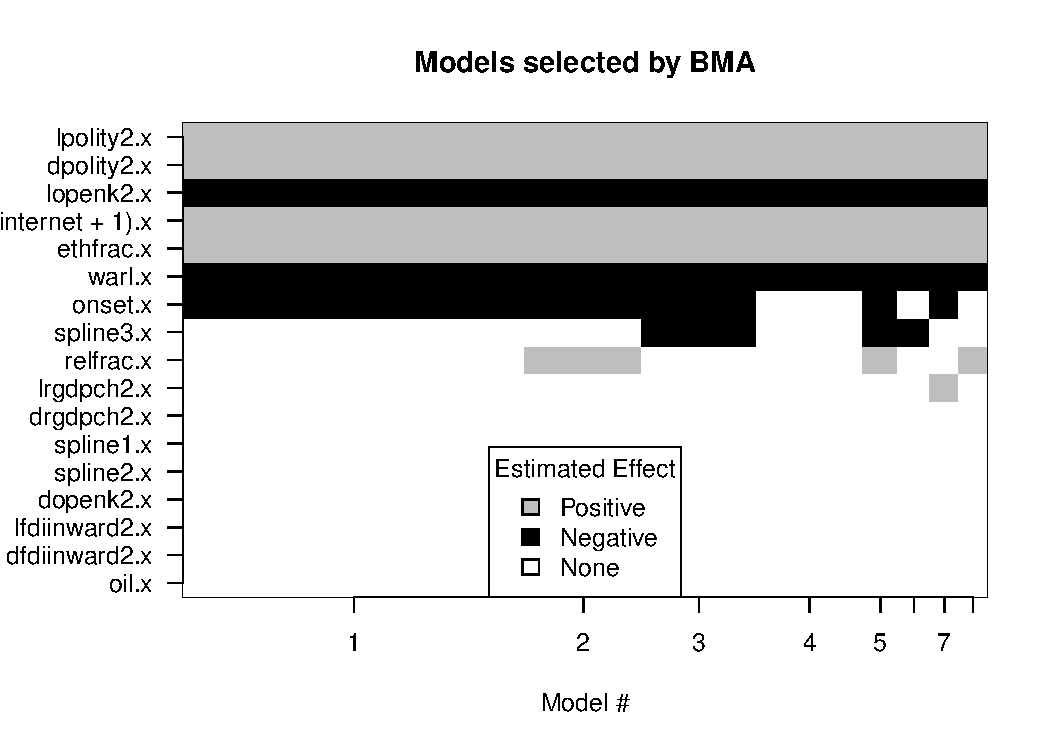
\includegraphics[width=\maxwidth]{figures/BMA_Plot_Supp} 

}



\end{knitrout}
  \end{center}
    \begin{singlespace}
        {\scriptsize{}}
    \end{singlespace}
\end{figure}
\clearpage
}

\afterpage{
\begin{figure}[t]
    \caption{BMA: Probabilities of inclusion (FPI removed)}
    \label{absolute}
    \begin{center}
\begin{knitrout}
\definecolor{shadecolor}{rgb}{0.969, 0.969, 0.969}\color{fgcolor}

{\centering 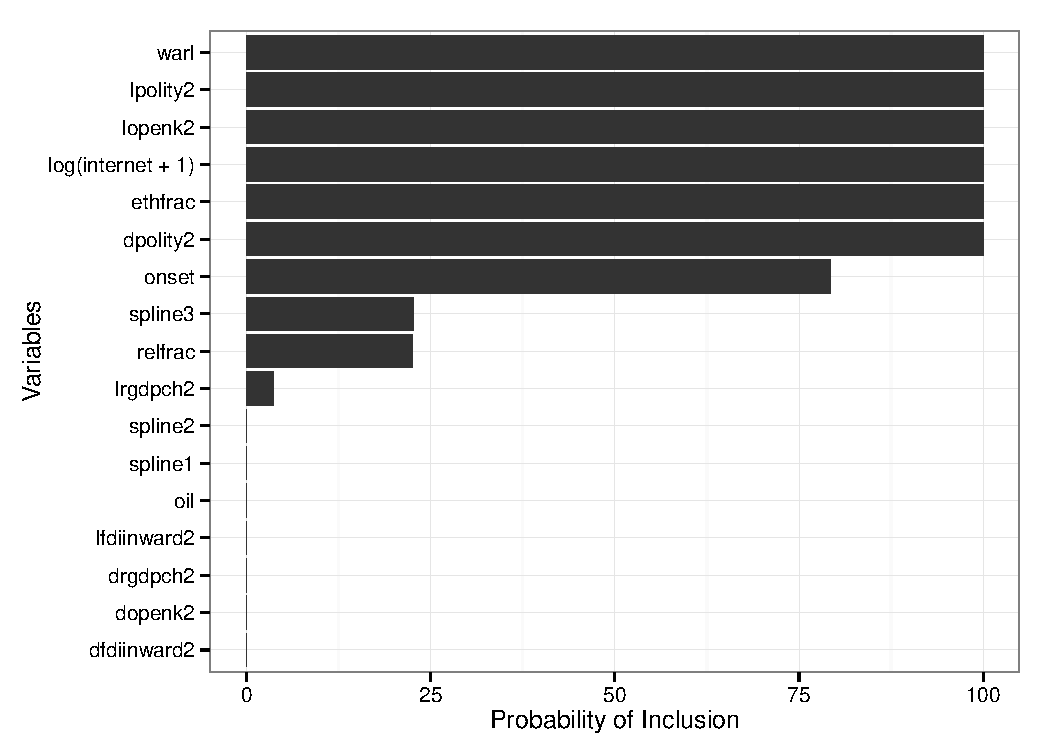
\includegraphics[width=\maxwidth]{figures/BMA_Plot_Supp_Inclusions} 

}



\end{knitrout}
  \end{center}
    \begin{singlespace}
        {\scriptsize{}}
    \end{singlespace}
\end{figure}
\clearpage
}


\begingroup
\setstretch{0.8}
\setlength\bibitemsep{7pt}

\xpatchbibmacro{date+extrayear}{%
  \printtext[parens]%
}{%
  \setunit{\addperiod\space}%
  \printtext%
}{}{}


\pagebreak
\printbibliography
\endgroup


\end{document}
